\section{Anforderungsanalyse}

Dieses Kapitel beschreibt die generellen Anforderungen an die Entwicklungsumgebung und einiger Beispielprojekte. Dabei werden auch einige theoretische Hintergründe betrachtet, speziell didaktische Konzepte für die Vermittlung von SQL oder mögliche Vorgehensweisen um Schüler bei der Entwicklung von Oberflächen sinnvoll anzuleiten. Den Schwerpunkt bildet die Beschreibung der beiden wichtigsten Komponenten der Entwicklungsumgebung: Den spezialisierten Editoren für SQL und Oberflächen.

Die hier ``erträumte'' Konzeption wird möglicherweise aufgrund der Endlichkeit der im Rahmen einer Master-Thesis zur Verfügung stehenden Zeitspanne nicht vollständig umgesetzt werden können. Trotzdem ist eine möglichst vollständige Erfassung von Anforderungen unerläßlich, um im Falle einer Fortführung der Entwicklung nicht aufgrund von unberücksichtigten Anforderungen große Umbauarbeiten vornehmen zu müssen. Die Planung konkreter Umsetzungsstrategien, inklusive einer Erläuterung der notwendigen Schnittstellen, werden in Kapitel \ref{sec:implementation-analysis}~\nameref{sec:implementation-analysis} besprochen. Sofern sich während der Entwicklung Ideen für bisher nicht bedachte Funktionalität ergaben, so wurden diese in Anlehnung an den ``Minus 100 Points''-Artikel von Eric Gunnerson \cite{gunnerson-minus-100} geprüft.

\info[inline]{Der Verzicht auf die technischen Hintergründe der Implementierung in diesem Kapitel soll es auch für ``normale'' Informatiklehrer verständlich machen, ohne Sie gleich mit den ``unwichtigen'' Details der Realisierung zu erschlagen.}

\subsection{Zielgruppe}
\label{sec:target-audience}

\missing[inline]{Fehlt noch, halt Schüler ohne vertiefte Mathe- oder Englischkenntnisse.}

\subsection{Grundprinzipien}
\label{sec:principles}

Nach der Betrachtung der zu bedienenden Zielgruppe und der Beschäftigung mit bereits existierenden Alternativen, ist es zunächst sinnvoll ein paar allgemeine Grundprinzipien zu formulieren. Diese Prinzipien bilden die Philosophie hinter der Schülerentwicklungsumgebung ab und dienen als Leitfaden für Designentscheidungen.

Praktisch erlaubt das vor allem eine relativ akkurate Abschätzung, ob sich die Implementierung einer bestimmten Idee lohnt und wie sie zu priorisieren ist. Diese Sortierung dieser Prinzipien ist entsprechend ihrer Bedeutung absteigend sortiert, das wichtigste Prinzip wird also zuerst genannt.

\begin{description}
\item[Semantik vor Syntax] \hfill\\
  Den Lernenden sollen kontextsensitiv sinnvolle Operationen angeboten werden, optimalerweise mit einer kurzen Erläuterung, warum gerade nur diese Teilmenge an Operationen möglich ist. Die eigentliche Programmierung erfolgt dann durch die Kombination von Bausteinen, ähnlich wie bei der Lernsoftware ``Scratch''. Durch kontinuirliches Feedback der Entwicklungsumgebung sollen die Lernenden in die Lage versetzt werden, auch ohne ständige Rückversicherung bei der Lehrkraft eigene Ansätze zu erproben. Syntaxfehler, ein typisches Problem für viele Anfänger, werden durch dieses Vorgehen konstruktiv verhindert.
\item[Motivation durch praktisch vorzeigbare Ergebnissen] \hfill\\
  Der Einstieg in die Programmierung ist oftmals von relativ langweiligen Programmen geprägt, häufig textbasierten Konsolenanwendungen, welche sich nicht gut im Freundes- oder Bekanntenkreis präsentieren lassen. Im Sonderfall der Vermittlung von SQL Kenntnissen ist das Ergebnis der Arbeit sogar überhaupt nicht sinnvoll zu demonstrieren, weil die erstellten Abfragen isoliert für sich stehen und häufig auch nur in der Entwicklungsumgebung der jeweiligen Datenbank ausführbar sind. Mit der im Rahmen dieser Arbeit zu erstellenden Software sollen sich hingen praktisch relevante, allerdings sehr datenorientierte Programme umsetzen lassen. Diese verfügen über von den Lernenden zusammengestellte Eingabemasken um Daten einzufügen oder zu manipulieren und verschiedene Ausgabesichten um den Datenbestand sinnvoll zu präsentieren.
\item[Schrittweise komplexere Benutzeroberfläche der Entwicklungsumgebung] \hfill \\
  Konventionelle Entwicklungsumgebungen sind Programme von Profis für Profis und bieten einen dementsprechend ausgerichteten Funktionsumfang. Gerade wenn man aber dabei ist etwas Neues zu lernen, kann es sinnvoll sein, die Menge der möglichen Optionen zu beschränken. In diesem Sinne sollte die Lehrkraft die Möglichkeit haben, den Funktionsumfang der Entwicklungsumgebung für Schüler gezielt zu reduzieren. Es sollten sich also Funktionen der Entwicklungsumgebung ausblenden lassen, wenn dies aus didaktischen Gründen sinnvoll erscheint. Zum Beispiel könnten bestimmte Bedienelemente oder Bestandteile von SQL ausgeblendet werden, wenn diese noch nicht behandelt worden sind.
\item[Einfache Inbetriebnahme] \hfill \\
  Eine initiale Hürde jeder (Lern-)Software ist deren Installation, insbesondere bei Programmen aus dem Datenbankumfeld. Die Inbetriebnahme der für Server konzipierten Programme auf privaten, ``normalen'' Rechnern führt immer wieder zu Problemen aufgrund von nicht aufgelösten Abhängigkeiten, fehlenden Rechten beim Starten von Systemdiensten oder bei Dateizugriffen. Die zunehmende Heterogenität an Betriebssystemen, insbesondere die zunehmende Verwendung MacOS \cite{statista-os-verbreitung}, tut ein Übriges um die Verteilung von Software zu erschweren. Damit der eigentliche Lernprozess nicht schon vor dem Start der Entwicklungsumgebung behindert wird, ist eine möglichst einfache Inbetriebnahme von entsprechender Bedeutung. Die Informatiklehrkräfte stehen bei dem Betrieb der jeweiligen Programme in der Schule vor ähnlichen Problemen wie ihre Schüler, nur dass Sie auf die Konfiguration des Rechnerpools ihrer Schule oftmals nur einen eingeschränkten Einfluss haben. Die im Vergleich zu privaten Rechnern wesentlich restriktiver gehandhabte Rechte eines Schul-PCs verkomplizieren dieses Szenario zusätzlich. Damit der Lernprozess mit esqulino nicht schon mit einer fehlgeschlagenen Installation endet, soll die Inbetriebnahme so wenig Hürden wie möglich aufstellen.
\item[Fortführung der entwickelten Projekte] \hfill \\
  Lernumgebungen wie Scratch oder der AppInventor sind in sich geschlossene Systeme, deren Arbeitsergebnisse nur schwer in anderen Programmen oder Kontexten von Nutzen sind. Sobald der Lernende dann die Grenzen der verwendeten Lernsoftware erreicht hat, steckt er in einem Dilemma: Es ist für ihn notwendig auf eine andere Software auszuweichen, in diese kann er sein bestehendes Projekt aber nicht einfach mitnehmen. Die Arbeitsergebnisse dieser zu entwickelnden Software sollen daher zumindest einfach einsehbar sein, optimalerweise nach einem Export sogar mit gängigen Entwicklungsumgebungen oder Texteditoren erweiterbar.
\end{description}

\subsection{Künftigen Erweiterungen vorbehalten}
\label{sec:out-of-scope}

Umgekehrt ist es auch wichtig, den Umfang des zu entwickelnden Programms auf einem im Rahmen der Thesis machbaren Umfang zu begrenzen. Die folgenden Ideen wären mehr oder minder naheliegende Ergänzungen, welche aufgrund der zur Verfügung stehenden Zeit aber nicht implementiert werden sollen\footnote{Die griffigere, englische Bezeichnung dafür wäre "`out of scope"', \href{http://german.stackexchange.com/questions/31085/german-equivalent-to-out-of-scope/}{dazu kennt allerdings auch das Internet keine direkte Übersetzung}}.

\begin{description}
\item[Datenmodellierung] \hfill \\
  Der Schwerpunkt dieser Arbeit liegt zunächst auf der Vermittlung von Kenntnissen zur Abfrage und Manipulation von Daten in einem bestehenden Schema. Änderungen an diesem Schema sind nicht vorgesehen, demzufolge ist auch der Neuentwurf eines Schemas mit externen Mitteln zu bewerkstelligen. Völlig außerhalb des Umfangs dieser Arbeit ist die Überführung von konzeptionellen Modellen (z.B. ER-Schemata) in physikalische Modelle.
\item[Aufwändiges Design von Benutzerschnittstellen] \hfill \\
  Auch wenn die Konzeption der Benutzerschnittstelle für die verschiedenen Masken in den eben aufgezählten Prinzipien auftaucht, ist es wichtig den engen Rahmen dieses Aspektes zu verstehen. Es geht um die Schaffung von einfachen, datenzentrierten Eingabemöglichkeiten, nicht um die Umsetzung besonders kreativer Bedienkonzepte. Dementsprechend ist z.B. die Erweiterung der zur Verfügung stehenden Eingabeelemente durch die Lernenden außerhalb des Rahmens dieser Arbeit.
\end{description}

\subsection{Allgemeines Konzept der Entwicklungsumgebung}
\label{sec:design-general-concept}

\missingfigure{UI-Konzept mit traditioneller "`Seitenleiste"' und "`Editorbereich"'}

Dieses Kapitel beschreibt sehr allgemein Anforderungen an die Entwicklungsumgebung, die Details dazu werden in den spezifischeren Kapiteln besprochen, welche nach Möglichkeit verlinkt sind.

\subsubsection{Zwei Modi: Entwickeln und Anschauen}

Grundsätzlich unterschieden werden muss bei der Schülerentwicklungsumgebung, ähnlich wie bei Scratch, zwischen zwei Betriebsmodi für ein Projekt: Zunächst wird ein Projekt im Entwicklermodus betrieben, in diesem Fall stehen dem Benutzer alle Entwicklungstools zur Verfügung. Wenn es dann später einmal fertig ist und an Endanwender, z.B. Bekannte oder Freunde, weitergegeben wird, erwarte diese natürlich eine normale Benutzeroberfläche zu sehen. Der Wechsel zwischen diesen beiden Modi sollte dabei, ebenfalls analog zu Scratch, zu jedem Zeitpunkt möglich sein. Der Weg von der Entwicklungsumgebung zum Programm ist dabei selbstverständlich, jedoch sollte nach Möglichkeit auch der "`Rückweg"' von der Endbenutzeroberfläche zur Entwicklungsumgebung jederzeit möglich sein. Das "`Verstecken"' von Vorgehensweisen in Projekten ist im Lehrbetrieb nicht vorgesehen, jedes fremde Projekt soll auch als Inspiration für die Umsetzung eigener Ideen dienen können.

\subsubsection{Webanwendung}

Um die einfachste Verwendung der Software für Lernende zu gewährleisten, wird esqulino als Webanwendung entwickelt. Für die ersten Schritte der Softwareentwicklung mit SQL reicht auf Seite der Lernenden dann ein beliebiger, aktueller Browser. Wie aus Kapitel \ref{sec:related-work} \nameref{sec:related-work} ersichtlich, befindet sich esqulino mit diesem Ansatz in guter Gesellschaft: Das ``große Vorbild'' Scratch ist über den Browser erreichbar, genau so wie auch die anderen explizit als Lernsoftware beschriebenen Anwendungen.

Selbstverständlich muss eine Entscheidung mit einer solchen Tragweite dennoch gut abgewogen werden. Das vergleichbare Arbeiten sich ebenfalls für diesen Ansatz entschieden haben ist zwar ein starkes Indiz, isoliert betrachtet aber natürlich keine stichhaltige Begründung. Immerhin existiert von Scratch auch eine lokal installierbare Fassung, welche der Entwicklung der Webversion allerdings leicht hinterherhinkt\footnote{\href{https://scratch.mit.edu/scratch2download/}{Scratch Download-Seite: "The backpack is not yet available."}}.

Praktisch bedeutet dieser Ansatz vor allem eine Verschiebung der Probleme mit der Inbetriebnahme auf die Lehrperson. Bei der Konzeption von esqulino wird davon ausgegangen, dass die Bereitstellung eines Serverdienstes in Zeiten von Virtualisierungs- und Containerumgebungen für Informatik-affine Lehrkräfte keine nennenswerte Hürde mehr darstellt.

Ebenfalls aus Gründen der einfacheren Zugänglichkeit sollte eine einzelne Serverinstanz in der Lage sein, mehrere Projekte simultan zu bedienen. Die Lehrperson kann also mit einem einzigen Serverprozess eine ganze Klasse versorgen. Eine Begleiterscheinung dieses zentralen Angebots ist allerdings die notwendige Implementierung von zumindest rudimentären Zugriffsbeschränkungen: im Normalfall sollen Schüler die Projekte ihrer Klassenkameraden zwar jederzeit begutachten, aber nicht modifizieren können. Würde die Entwicklungsumgebung von den Schülern lokal betrieben, entfiele die unmittelbare Notwendigkeit einer Zugriffsbeschränkung.

Durch den Betrieb eines zentralen Servers für die Projekte der Schüler entfällt auch eine weitere typische Problemquelle im Unterichtsalltag: Sofern der Server tatsächlich durchgehend betrieben wird, ist es sehr einfach auch von zuhause an den Projekten weiter zu arbeiten. Die Notwendigkeit manuell Dateien über USB-Sticks, Netzlaufwerke oder sonstige Dienste zu synchroniseren entfällt.

Ein weiterer Vorteil eines zentralen Servers ergibt sich in der praktischen Vorzeigbarkeit der eigenen Ergebnisse: Durch einfache Weitergabe der URL für Endbenutzer können die Lernenden ihre entwickelten Applikationen mit Eltern, Freunden und anderen Personen teilen.

Nicht verschwiegen werden sollen allerdings auch die negativen Nebeneffekt dieser grundsätzlichen Entscheidung: Zunächst einmal wird dadurch ein eigenständiger Betrieb der Entwicklungsumgebung durch Schüler deutlich erschwert. Diese müssten auf ihrem eigenen Rechner plötzlich doch eine Server-Instanz betreiben, anstatt einfach ein Programm zu starten. Faktisch wird die Bereitstellung einer dezidierten Umgebung für den Server also zur Pflichtaufgabe der jeweiligen Lehrperson. Vom Betrieb eines dedizierten Servers in der Schule, über die Verwendung eines ``privat greifbaren'' Servers der Lehrperson bis hin zur Verwendung einer Cloud-Computing-Instanz im Internet sind unterschiedlichste Szenarien denkbar. Der erfolgreiche Einsatz von esqulino hängt in der Praxis dann aber auch maßgeblich von der Verfügbarkeit dieses Serverdienstes ab.

Softwaretechnisch nachteilig ist die Tatsache, dass esqulino im Falle einer Entwicklung als ``traditionelle Desktopawendung'' auf ein großes Ökosystem aus bestehenden Entwicklungsumgebungen zurückgreifen könnte. Jede größere Entwicklungsumbegung (Eclipse, Visual Studio, ...) bietet eine Plugin-Schnittstelle, auf die man mit esqulino hätte aufsetzen können. Ähnlich gut erprobte Umgebungen für Browser gibt es hingegen leider nicht, es müssen daher relativ viele technisch Kleinigkeiten (Toolbars, Projektbrowser, ...) extra für esqulino entwickelt werden.

\subsubsection{Projektbasiert}

Nachdem der Begriff des ``Projekts'' nun schon einige Male gefallen ist, wird es Zeit diesen eindeutig zu definieren. Abstrakt betrachtet handelt es sich bei einem Projekt um eine Datenbasis in Form einer Datenbank. Zu dieser Datenbasis kann man als Entwickler SQL-Abfragen entwickeln (\ref{sec:design-sql-editor} \nameref{sec:design-sql-editor}) und einige dieser Abfragen mit einer Oberfläche für Endbenutzer versehen (\ref{sec:design-ui-editor} \nameref{sec:design-ui-editor}).

Als unmittelbare Ausgangspunkt eines Projektes sollen einigermaßen einfache, aber grundsätzlich beliebige SQLite-Datenbanken dienen\footnote{Kapitel \ref{sec:implementation-database-system} \nameref{sec:implementation-database-system} erläutert, warum ausgerechnet SQLite zum Einsatz kommt und nicht ein anderes DBMS.}. Diese Schemata werden vorher mit externen Programmen erzeugt, was sowohl im Dialog mit den Schülern als auch ``einfach so'' erfolgt sein kann.

Im Sinne einer möglichst niedrigen Einstiegshürde soll es den Anwendern leicht gemacht werden, bestehende Projekte zu übernehmen. Im Informatikunterricht müssen häufiger zu Beginn bestimmte Schritte ausgeführt werden, ``weil das nun mal so ist'' (also eine ausführliche Erklärung zu diesem Zeitpunkt zu weit gehen würde). Im Falle des Sprachumfangs von SQL ist das zwar im Vergleich zu z.B. Java nicht ganz so dramatisch\footnote{``Herr Lehrer, was macht eigentlich dieses \texttt{public static void}?''}, aber nach Möglichkeit zu vermeiden.

Dementsprechend sollte normalerweise jeder Schritt beim Anlegen eines neuen Projektes für die Schüler nachvollziehbar sein. Wenn dann aber doch einmal eine Serie von ``mechanisch auszuführenden'' Anweisungen erforderlich sein sollte, wäre es aber dennoch praktisch, diesen Vorgang durch eine Kopie eines schon bestehenden Projektes abzukürzen. Die Lehrkraft würde in diesem Fall ein Projekt für ihre Schüler vorbereiten, welches diese dann mit einem Klick in ein anders benanntes Projekt kopieren können. Es werden dann alle Bestandteile, möglicherweise mit einer einfachen Anpassung der Zugriffsrechte, unter dem neuen Namen verfügbar gemacht.

\subsubsection{Zugriffskontrollen}

Lesende Zugriffe können, zumindest in der Thesis-Version der Software, nicht endgültig eingeschränkt werden. Natürlich könnte man theoretisch typische Entwurfsmuster für Zugangsbeschränkungen auch in esqulino implementieren: Auf einfachster Ebene wäre zum Beispiel denkbar, dass eine Spalte "`geheim"' zu Tabellen mit privaten Daten hinzugefügt wird und auf dieser Basis die Oberfläche für Endanwender solcherart markierte Daten nicht anzeigt. Da Projekte aber auch einfach kopiert werden können, müsste ein versierter Benutzer nur eine Kopie des Projektes vornehmen und könnte dann über den Editor alle Daten einsehen oder auch den Zugriffschutz der Oberflächen einfach deaktivieren. Um also den lesenden Zugriff effektiv zu verhindern müsste die Einsicht in die Quellen fremder Projekte eingeschränkt werden. Selbstverständlich wäre es mit entsprechendem Zeitaufwand prinzipiell möglich ein hinreichend sicheres System für den speziellen Anwendungsfall von esqulino zu entwerfen, dieser Aufwand wäre jedoch im Vergleich zu anderen Features nicht zu rechtfertigen. Und abgesehen davon sollte kein Schüler einem esqulino-Server Daten anvertrauen, deren versehentliche Veröffentlichung er oder sie nicht verkraften würde. Das gilt selbstverständlich auch für den Fall, dass eine hypothetische künftige Version einen solchen Zugriffsschutz vorsehen sollte!

Schon um Vandalismus zu vermeiden, sind leider einfache Zugriffskontrollen auf Projektebene nötig. Um etwaige Missverständnisse von vornerein zu vermeiden: Ziel dieser Kontrollen ist es zu verhindern, dass z.B. die Quellen für die Abfragen oder Benutzeroberfläche eines Projektes entstellt oder gelöscht werden. \textbf{Nicht geschützt} werden damit einzelne Datensätze, also die Zeilen, in der Datenbank. Sobald in der Benutzeroberfläche für Endanwender Funktionalität zum Löschen oder Editieren von Datensätzen vorgesehen ist, gibt es keine einfache Möglichkeit, legitime Veränderungen von unerwünschtem Vandalismus zu unterscheiden. Daher soll zunächst nur eine sehr einfache, binäre Klassifikation in zwei Benutzergruppen vorgenommen werden: "`Darf jede mutierende Operation ausführen"' oder "`darf ausschließlich lesen"'. In einer späteren Version wäre es dann denkbar diese sehr grobe Methodik zu verfeinern.

Sowohl für den lesenden als auch für den schreibenden Zugriff gilt daher: Eine komplexe, aber halbgare Lösung für eine so kritische Funktionalität würde im Extremfall mehr Schaden anrichten als nützen. Eine unsicher implementierte Sicherheitsfunktion suggeriert möglicherweise ein Schutzniveau welches praktisch nicht eingehalten wird. Also werden Ansätze wie "`Vergabe von Schreibrechten für einzelne Abfragen an bestimmte Benutzergruppen"' oder sogar ein zeilenweiser Schutz von Daten ("`Jeder Benutzer darf nur seine Daten bearbeiten"') aus Zeitgründen im Rahmen dieser Thesis nicht weiter betrachtet.

Trotzdem ist es leider notwendig zumindest eine grundlegende Form von Authentifizierung vorzusehen. Diese Notwendigkeit ergibt sich auf zwei Ebenen: Es sollen sowohl der Code als auch die Datenbestände vor Veränderungen durch unbefugte Dritte geschützt. Dabei muss es sich nicht einmal um bösartigen Vandalismus handeln. Bei ungeschickt programmierten Webseiten kann es durchaus auch mal passieren, dass Webcrawler Datenbestände vernichten. Mehr als einen schlecht ausprogrammierten "`Diesen Datensatz Löschen"'-Link auf einer Übersichtsseite braucht es dazu nicht. Der Webcrawler folgt unter Umständen auch solchen Verweisen und löscht damit während der Indexierung unbeabsichtigt Datensätze.

Um also zumindest einen grundsätzlichen Schutz zu ermöglichen, sollten für ein Projekt zwischen drei schreibenden Zugriffsarten für angelegte Benutzer gewählt werden können:

\warning{Nur zur Sicherheit sei an dieser Stelle nochmals deutlich erwähnt, dass dieser Schutz nur für schreibende Zugriffe greift. Der lesende Zugriff auf den gesamten Datenbestand ist über die Entwicklungsumgebung auch für Gäste stets uneingeschränkt möglich.}

\begin{description}
  \item[Entwickler] \hfill \\
    Mit diesem Zugangslevel hat ein legitimierter Benutzer das Recht beliebige Änderungen an dem Projekt vorzunehmen. Dabei ist es egal, ob er mit der Entwicklungsumgebung oder der Oberfläche für Endbenutzer arbeitet.
  \item[Benutzer] \hfill \\
    Diese Personengruppe hat keine Möglichkeit den Quelltext eines Projektes zu editieren, kann aber uneingeschränkt auf die Funktionalität der Oberfläche für Endbenutzer zugreifen. Sofern z.B. das Löschen von bestimmten Datensätzen über die Oberfläche für Endbenutzer nicht möglich ist, können diese Daten von dieser Personengruppe auch nicht gelöscht werden.
  \item[Gast] \hfill \\
    Gäste können keinerlei Schreibzugriffe vornehmen, weder über die Entwicklungsumgebung, noch über die Oberfläche für Endbenutzer.
\end{description}

\subsection{Didaktisch sinvolle Teilmengen von SQL}
\label{sec:sql-subset}

\warning{Nicht alle hier beschriebenen Optionen sind notwendigerweise in der Entwicklungsumbegung implementiert! Dieses Kapitel ist eine \textit{allgemeine} Betrachtung von didaktisch sinnvollen Teilmengen von SQL. Um zu sehen, welche Funktionalität tatsächlich implemtiert worden ist lohnt sich ein Blick in Anhang \ref{app:implemented-features}:~\nameref{app:implemented-features}.}

Die uneingeschränkte Umsetzung des SQL-Standards würden sowohl für den Verfasser dieser Arbeit als auch für die Anwender der Entwicklungsumgebung viele unpraktische Probleme aufwerfen. Der SQL-Sprachumfang ist mittlerweile gewaltig und die Anzahl der verschiedenen Dialekte unüberschaubar groß. Varianten wie Transact-SQL bieten die Möglichkeit zur Laufzeit mit Schleifen, Fallunterscheidungen und Variablen zu arbeiten und erfüllen damit alle Kriterien für Turing-Vollständigkeit. Darüber hinaus werden ``echte'' Entwicklungsumgebungen für SQL von großen Entwicklerteams konzipiert und programmiert, der Autor dieser Arbeit bildet hingegen ein (immerhin motiviertes) Ein-Mann-Team.

Glücklicherweise wäre aber auch der Zielgruppe dieser Entwicklungsumgebung mit einer vollständigen Umsetzung des SQL-Standards überhaupt nicht gedient. Im Gegensatz zu allen anderen Entwicklungsumgebungen da draußen soll die Stärke dieser Entwicklungsumgebung in einer sinnvollen Reduktion liegen. Dieses Kapitel beschreibt daher, wie man zum ``normalen'' SQL kompatible Untermengen definieren kann, um einige spezifische Aufgaben zu erfüllen. Oder in Anlehnung an die "`80/20"'-Regel ausgedrückt: Es gilt jene 20\% des Sprachumfangs abzubilden, mit denen sich 80\% der typischen Aufgaben gut lösen lassen. Vor diesem Hintergrund dient dieses Kapitel also ebenfalls als Grundlage für die Entscheidung den SQL-Editor im Rahmen dieser Arbeit als "`abgeschlossen"' zu betrachten.

Bei einer gängigen Programmiersprache wie z.B. Java bauen die einzelnen Sprachfeatures sehr viel stärker aufeinander auf, es ergeben sich deutlich weniger Reihenfolgen in denen man diese sinnvoll aktivieren könnte. Die wesentlich größere Standardbibliothek einer solchen Sprache trägt dann ebenfalls dazu bei, die Suche nach voneinander weitestgehend unabhängig funktionierenden Teilsprachen zu erschweren.

Glücklicherweise erlaubt die Struktur von SQL die Verwendung von sehr lokalen Einschränkungen, deren Auswirkungen sich gut abschätzen lassen. Einzig der Umgang mit Ausdrücken überspannt fast alle Bereiche von SQL: Diese können an sehr vielen Stellen auftreten und müssen dementsprechend sorgfältig analysiert werden. Durch diese vergleichsweise überschaubaren Abhängigkeiten ergeben sich viele mögliche Reihenfolgen in denen man Sprachfeatures aktivieren kann. Ohne zu diesem Zeitpunkt weiter auf die Vor- und Nachteile der jeweiligen Reihenfolgen einzugehen, wären die folgenden Varianten zumindest denkbar:

\begin{itemize}
  \item Filterung von Daten mit komplexen logischen Ausdrücken, zum Beispiel unter Verwendung des \texttt{LIKE}-Operators, Kombinationen mit \texttt{AND} oder \texttt{OR}, geschachtelte Ausdrücke mit mathematischen Anweisungen, ...
  \item Kombination von Daten in unterschiedlichen Tabellen mittels \texttt{JOIN}-Operationen.
  \item Aggretation von Daten mit dem \texttt{GROUP BY}-Operator und den aggregierenden Funktionen.
  \item Projektion von Daten mit Ausdrücken und Funktionen innerhalb der \texttt{SELECT}-Komponente.
\end{itemize}

Es soll nicht Aufgabe von esqulino sein, diese unterschiedlichen Reihenfolgen implizit zu bewerten, in dem eine "`beste"' Variante fest eingebaut wird. Viel mehr sollen die Lehrkräfte in die Lage versetzt werden, je nach verwendetem Lehrmaterial zu entscheiden, welcher Umfang dafür angemessen ist. Wir klären in diesem Kapitel daher zunächst, welche Features von SQL überhaupt für die Entwicklungsumgebung von Belang sind und wie diese voneinander abhängen.

\subsubsection{Mögliche Einschränkungen der Komponenten}
\label{sec:sql-subset-local}

Die folgende Beschreibung untersucht zunächst nur die Komponenten einer \texttt{SELECT}-Suchanfrage. Diese sind, im Gegensatz zu \texttt{DELETE}, \texttt{UPDATE} und \texttt{INSERT} nicht auf eine Tabelle beschränkt und auch von der schieren Anzahl der verfügbaren Optionen her deutlich mächtiger.

Zunächst definieren wir einige mögliche Einschränkungen anhand der grundlegenden Struktur jeder suchenden SQL-Abfrage. Da die Reihenfolge der Komponenten nicht beliebig ist, ergibt sich eine sehr klare Struktur in der einige Komponenten auch allerdings übersprungen werden können. Abbildung \ref{fig:sql-steps} wurde aus den Vorlesungsunterlagen von Prof. Dr. Hoffmann entnommen und demonstriert den logischen Ablauf bei der Verarbeitung einer SQL-Abfrage inklusive aller Zwischenschritte und optionaler Komponenten. Daraus ist folglich gut ersichtlich, dass alle Komponenten einer Suchanfrage bis auf die logisch Erste (\texttt{FROM}) und Letzte (\texttt{SELECT}) optional sind.

\begin{figure}
  \centering 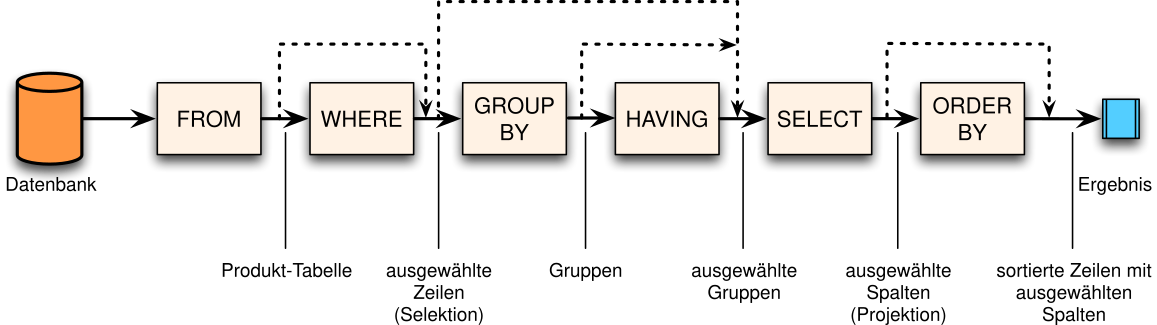
\includegraphics{images/sql-steps.png}
  \caption{Komponenten und sich ergebende Zwischenschritte bei der Verarbeitung einer SQL-Abfrage von Prof. Dr. Ulrich Hoffmann.}
  \label{fig:sql-steps}
\end{figure}

Einige der im folgenden beschriebenen Optionen sind redundant. Das liegt zum einen an SQL selbst, die Sprache sieht schlichtweg mehrere syntaktische Varianten für semantisch äquivalente Sachverhalte vor. Zum anderen könnte es aber auch aus didaktischen Gründen sinnvoll sein, die Wissensvermittlung mit einer Reihe von Spezialfällen zu beginnen.

\begin{enumerate}
\item \textbf{Projektionen mit \texttt{SELECT}} \\
  Diese Komponente als solche kann für Suchabfragen nicht ausgeschlossen werden. Außerdem muss mindestens \ref{feat:select-all} $\lor$ \ref{feat:select-column} erlaubt sein, sonst können keine gültigen SQL-Abfragen erstellt werden.
  \begin{enumerate}
  \item \label{feat:select-all} Auswahl aller Spalten (``Sternchen-Operator'' \texttt{SELECT *})
  \item \label{feat:select-column} Auswahl von Spalten
  \item \label{feat:select-single-function} Ausdrücke aus einfachen Funktionsaufrufen zulassen
  \item \label{feat:select-simple-expression} Einfache Ausdrücke zulassen.
  \item \label{feat:select-expression} Beliebige Ausdrücke zulassen.
  \item \label{feat:select-distinct} Filterung des Ergebnisses auf unterscheidbare Daten (\texttt{DISTINCT}).
  \item \label{feat:select-limit} Beschränkung der Datenmenge mit \texttt{LIMIT}
  \end{enumerate}
\item \textbf{Angabe von Datenquellen mit \texttt{FROM}} \\
  Auch die Auslassung dieser Komponente ist nicht zulässig, obwohl einige SQL Dialekte dies durchaus erlauben. Im Rahmen von esqulino wird dies aber nicht unterstützt: Die Schüler sollen SQL Abfragen grundsätzlich auf Tabellen beziehen und keine Daten ``aus der Luft greifen''\footnote{Für Oberflächen werden manchmal noch so etwas wie globale Konstanten benötigt, diese kommen dann aber nicht aus der SQL-Schicht.}.
  \begin{enumerate}
  \item \label{feat:from-cross-join} Kreuzprodukt (\texttt{JOIN}) zulassen
  \item \label{feat:from-cross-comma} Kreuzprodukt (komma-separierte Schreibweise) zulassen
  \item \label{feat:from-natural-join} Automatische innere Verknüpfung zulassen (\texttt{NATURAL JOIN})
  \item \label{feat:from-inner-join} Innere Verknüpfung zulassen (\texttt{INNER JOIN}), erfordert \ref{feat:from-using} $\lor$ \ref{feat:from-on-simple}
  \item \label{feat:from-left-join} Linke äußere Verknüpfung zulassen (\texttt{LEFT OUTER JOIN}), erfordert \ref{feat:from-using} $\lor$ \ref{feat:from-on-simple}
  \item \label{feat:from-right-join} Rechte äußere Verknüpfung zulassen (\texttt{RIGHT OUTER JOIN}), erfordert \ref{feat:from-using} $\lor$ \ref{feat:from-on-simple}
  \item \label{feat:from-full-join} Volle äußere Verknüpfung zulassen (\texttt{FULL OUTER JOIN}), erfordert \ref{feat:from-using} $\lor$ \ref{feat:from-on-simple}
  \item \label{feat:from-using} \texttt{USING}-Bedingung zulassen
  \item \label{feat:from-on-simple} \texttt{ON}-Bedingung mit einfachen Ausdrücken zulassen
  \item \label{feat:from-on-expression} \texttt{ON}-Bedingung mit beliebigen Ausdrücken zulassen
  \item \label{feat:from-sub} Unterabfragen zulassen
  \end{enumerate}
\item \textbf{Filterung mit \texttt{WHERE} und \texttt{HAVING}} \\
  Da an dieser Stelle Ausdrücke zum Einsatz kommen, sind prinzipiell zwei unterschiedliche Ansätze denkbar. Zum einen die Verwendung einer vordefinierten Menge an Vergleichen mit einer einfachen Struktur, diese werden in \ref{sec:sql-subset-expression} beschrieben. Dem gegenüber steht der Ansatz fast beliebige Ausdrücke zu erlauben, was auf der einen Seite einen Ausbruch aus einem zu simplen Schema gleichkommen kann, auf der anderen Seite möglicher aber auch den Lernenden mit einem zu großen Freiheitsgrad überfordert.
  \begin{enumerate}
  \item \label{feat:where-allow} \texttt{WHERE} zulassen
  \item \label{feat:having-allow} \texttt{HAVING} zulassen
  \item \label{feat:where-and} Verknüpfungen mit \texttt{AND}
  \item \label{feat:where-or} Verknüpfungen mit \texttt{OR}
  \item \label{feat:where-simple-expression} Einfachen Ausdrücke zulassen
  \item \label{feat:where-expression} Beliebige Ausdrücke zulassen
  \end{enumerate}
\item \textbf{Bildung von Gruppen mit \texttt{GROUP BY}}
  \begin{enumerate}
  \item \label{feat:group-allow} \texttt{GROUP BY} zulassen
  \item \label{feat:group-multiple} Grupperierung mehrerer Spalten zulassen
  \end{enumerate}
\item \textbf{Sortierung mit \texttt{ORDER BY}} \\
  Bei dieser Komponente fehlt bewusst die Möglichkeit anhand eines Spaltenindexes aus dem \texttt{SELECT} zu sortieren. Da die gute Lesbarkeit der Abfragen ein erklärtes Ziel der Entwicklungsumgebung ist, wurde auf diese redundante Möglichkeit der Spaltenauswahl verzichtet.
  \begin{enumerate}
  \item \label{feat:order-allow} \texttt{ORDER BY} zulassen, die Auswahl der Richtung (\texttt{ASC} und \text{DESC}) ist dann grundsätzlich möglich
  \item \label{feat:order-select} Sortierung nach im \texttt{SELECT} erwähnten Spalten oder Ausdrücken zulassen
  \item \label{feat:order-any-column} Sortierung nach beliebigen Spalten zulassen
  \item \label{feat:order-expression} Sortierung anhand eines beliebigen Ausdrucks zulassen
  \end{enumerate}
\end{enumerate}

\subsubsection{Mögliche Einschränkungen der Ausdrücke}
\label{sec:sql-subset-expression}

Nach dieser Betrachtung der mit der unmittelbaren SQL-Struktur zusammenhängenden Funktionalität ist es nun an der Zeit, sich den Ausdrücken ausführlicher zu widmen. Um eine graduelle Lernkurve sowie eine sinnvolle Unterstützung durch den Editor zu gewährleisten, werden diese in drei Klassen eingeteilt:

\begin{description}
\item[Einfache Ausdrücke] \hfill\\
  Einfache Ausdrücke unterliegen einer ganz festen Struktur, die nur sehr begrenzt die Schachtelung oder Verkettung von zusammengesetzten Ausdrücken zulässt. Ziel dieser Reduktion ist, dass die Auswertungsreihenfolge dieser Ausdrücke auch ohne die Verwendung von Klammern ``intuitiv'' eindeutig ist.
  
  Die Bearbeitung dieser Ausdrücke ist nicht notwendigerweise völlig frei, sondern könnte auch hinsichtlich der möglichen Operatoren oder der Struktur eingeschränkt werden.
\item[Komplexe Ausdrücke] \hfill\\
  Komplexe Ausdrücke lassen sich schachteln bzw. verketten und können mit einem Scratch-ähnlichen Editor für Ausdrücke frei bearbeitet werden. Die korrekte Beachtung von Auswertungsreihenfolgen ist Aufgabe der Lernenden, weswegen diese ggfs. die Ausdrücke auch selber Klammern müssen.

\item[Beliebige Ausdrücke] \hfill\\
  Beliebige Ausdrücke werden textuell notierte und vom SQL-Editor nicht weiter geprüft, sondern ungefiltert in die Abfrage eingesetzt werden. Sofern diese Art von Ausdrücken zugelassen wird erfolgt also auch keinerlei inhaltliche Einschränkung der zur Verfügung stehenden Möglichkeiten oder eine Syntaxüberprüfung.

  Diese Option soll es besonders fortgeschrittenen Lernenden erlauben, auch in nicht von esqulino unterstützte Szenarien noch weiterarbeiten zu können. Damit wird verhindert, dass zu große Fortschritte der Lernenden esqulino sofort obsolet machen.
\end{description}

Mit dieser Unterscheidung im Hinterkopf, können wir nun eine Menge an didaktisch sinvollen Einschränkungen definieren. Die Schüler sollen dabei durchaus auch Lernen, dass es sich bei Ausdrücken (nicht nur in SQL) um ein allgemeines Konzept handelt, welches Prinzipiell in der \texttt{SELECT}-Komponente genau so angewandt werden kann wie beim \texttt{ORDER BY}. Oder plastisch ausgedrückt: Wenn sich die Schüler aus didaktischen Gründen erstmal nur mit Ausdrücke im Rahmen der \texttt{SELECT}-Komponente beschäftigen sollen ist das eine sinnvolle, und daher mögliche Einschränkung. Nicht sinnvoll hingegen wäre es die Anwendung der \texttt{LENGTH(X)} Funktion nur in einer der beiden Komponenten zuzulassen. Letzteres wird daher auch nicht unterstützt.

\begin{enumerate}
\item \textbf{Allgemeine Optionen} \\
  Diese Optionen betreffen prinzipiell alle Stellen, an denen die entsprechenden Arten von Ausdrücken zugelassen werden.
  \begin{enumerate}
  \item \label{feat:expr-allow-any-text} Ausdrücke als beliebigen Text zulassen, diese Option erlaubt die Umgehung aller Einschränkungen für einfache Ausdrücke!
  \item \label{feat:expr-allow-placeholder} An Stelle von Konstanten auch die Verwendung von Platzhaltern zur Bindung von Daten aus der Oberfläche zulassen.
  \end{enumerate}

\item \label{feat:expr-compute}  \textbf{Einfache Berechnende Ausdrücke} \\
  Diese Ausdrücke tauchen normalerweise in \texttt{SELECT}- oder \texttt{ORDER BY}-Komponenten auf, möglicherweise aber auch als Bestandteil eines einfachen Vergleichs.
  \begin{enumerate}
      \item \label{feat:expr-compute-simple-func} Einfacher Funktionsaufruf mit Spalten oder Konstanten als Argument
      \item \label{feat:expr-compute-simple-arithmetic} Einfache Rechenausdrücke mit einer mathematischen Operation ($alter + 1$, $anzahl * preis$)
      \item \label{feat:expr-compute-simple-concat} Konkatenation von Strings\footnote{Sofern auch eine Oberfläche entwickelt werden soll, ist eine Konkatenation im Regelfall lieber dort vorzunehmen.}
  \end{enumerate}

\item \textbf{Einfache Vergleichende Ausdrücke} \\
  Diese ``typischen'' Vergleichsausdrücke sollten ausreichen um einen Großteil der nötigen Vergleiche in \texttt{WHERE}, \texttt{HAVING} und \texttt{ON} Komponenten abzudecken. Die linke Seite dieser Ausdrücke ist stets eine zur Verfügung stehende Spalte, der Vergleichsoperator und die rechte Seite eine der hier aufgezählten Möglichkeiten.

  Mit Vergleich ist dabei nicht nur der $=$-Operator gemeint, sondern auch die relationen Operatoren $\ne, <,\ge,\le$ und $>$. Die komplexeren Operatoren \texttt{LIKE} und \texttt{IN} sowie der ternäre Operator \texttt{BETWEEN} werden aber gesondert aufgeführt.

  \missing[inline]{Testen wie weit man mit diesen einfachen Ausdrücken bei den Aufgaben von SqlZoo oder der Übung Datenbanken kommt.}
  \begin{enumerate}
  \item \label{feat:expr-compare-const} Vergleich einer Spalte mit einem konstanten Wert
  \item \label{feat:expr-compare-null} Vergleich einer Spalte gegen \texttt{NULL}
  \item \label{feat:expr-compare-other-col} Vergleich einer Spalte mit einer anderen Spalte
  \item \label{feat:expr-compare-simple-func} Vergleich einer Spalte mit einem einfachem berechnenden Ausdruck (siehe \ref{feat:expr-compute})
  \item \label{feat:expr-compare-between} Test einer Spalte mit dem \texttt{BETWEEN}-Operator und zwei Konstanten
  \item \label{feat:expr-compare-like} Nutzung des \texttt{LIKE}-Operators mit einer Konstanten
  \item \label{feat:expr-compare-in} Nutzung des \texttt{IN}-Operators mit einer Liste von Konstanten
  \item \label{feat:expr-compare-negate} Negation aller einfachen Ausdrücke
  \end{enumerate}

\item \textbf{Allgemeine Funktionen (in alphabetischer Reihenfolge)} \\
  In einem Umfeld für Anfänger ist zu erwarten, dass fast jede Funktion (bzw. jede logische Gruppe an Funktionen) einer eigenen Einführung bedarf. Die Lehrkräfte sollen diese daher isoliert zur Verfügung stellen können, ohne Ablenkung durch nicht benötigte Funktionen.

  Bei unterschiedlich überladene Varianten der gleichen Funktion wird in esqulino immer nur die vollständigste Variante implementiert. Die Schüler müssen daher nicht die implizit bekannten Werte der jeweiligen Funktion auswendig kennen.
  \begin{enumerate}
  \item \label{feat:fun-abs} \texttt{ABS(X)} um den Betrag eines Wertes zu erhalten.
  \item \label{feat:fun-coalesce} \texttt{COALESCE(X,Y,...)} um den ersten gültigen Wert der Parameterliste zu erhalten.
  \item \label{feat:fun-length} \texttt{LENGTH(X)} um die Länge einer Zeichenkette zu bestimmen.
  \item \label{feat:fun-casing} \texttt{LOWER(X)} und \texttt{UPPER(X)} um die klein bzw. groß geschriebene Variante einer Zeichenkette zu erhalten.
  \item \label{feat:fun-random} \texttt{RANDOM()} um einen zufälligen Wert zu erhalten.
  \item \label{feat:fun-round} \texttt{ROUND(X,Y)} um kaufmännisch zu runden.
  \item \label{feat:fun-trim} \texttt{TRIM(X)} sowie \texttt{LTRIM(X)} und \texttt{RTRIM(X)} um Leerzeichen am Anfang oder Ende eines Strings zu entfernen.
  \item \label{feat:fun-substr} \texttt{SUBSTR(X,Y,Z)} um einen Ausschnitt der Zeichenketten zu extrahieren.
  \item \label{feat:fun-replace} \texttt{REPLACE(X,Y,Z)} um Teilbereiche der Zeichenkette zu ersetzen.
  \item \label{feat:fun-instr} \texttt{INSTR(X,Y,Z)} um das Vorkommen eines Suchwortes in einer Zeichenkette zu erhalten.
  \end{enumerate}

\item \textbf{Aggregierende Funktionen (in alphabetischer Reihenfolge)} \\
  Die Verfügbarkeit dieser Funktionen hängt von der Verfügbarkeit der \texttt{GROUP BY}-Komponente ab (\ref{feat:group-allow}).
  \begin{enumerate}
  \item \label{feat:fun-avg} \texttt{AVG(X)} bildet das arithmetische Mittel.
  \item \label{feat:fun-count} \texttt{COUNT(X)} zählt alle Werte die nicht \lstinline{NULL} sind.
  \item \label{feat:fun-group-concat} \texttt{GROUP\_CONCAT(X,Y)} konkateniert einzelne Zellen einer Gruppe.
  \item \label{feat:fun-max-min} \texttt{MAX(X)} und \texttt{MIN(X)} selektieren minimalen oder maximalen Wert.
  \item \label{feat:fun-sum} \texttt{SUM(X)} summiert und gibt im Falle von komplett fehlenden Werten \texttt{NULL} zurück
  \item \label{feat:fun-total} \texttt{TOTAL(X)} summiert und gibt im Falle von komplett fehlenden Werten \texttt{0.0} zurück
  \end{enumerate}
\end{enumerate}

\subsubsection{Sprachstufen}
\label{sec:sql-subset-ranks}

Angelehnt an die bei Dr. Schemee bzw. Racket umgesetzte Idee der Feature-Levels \cite{macht-der-abstraktion} beschreibt dieses Kapitel konzeptionell, wie Lehrkräfte, aufbauend auf den im vorigen Kapitel beschriebenen Features, sinnvolle Untermengen von SQL definieren könnten, auf denen die mitgelieferten Beispielprojekte aufbauen. Bei den hier aufgeführten Beispielen handelt es sich keineswegs um die "`einzig korrekten"' Varianten. Vielmehr soll es für Lehrkräfte möglich sein, fast beliebige Teilmengen von SQL für ihre Schüler vorzugeben, nicht nur die im Rahmen dieser Arbeit als sinnvoll erachteten Kombinationen.

Das grundsätzliche Vorgehen um den Sprachumfang einzuschränken, ist dabei mehrstufig. Initial wird auf Projektebene mit einer Whitelist gearbeitet: Jede explizit erlaubte Funktionalität steht im SQL-Editor (siehe Kapitel \ref{sec:design-sql-editor} \nameref{sec:design-sql-editor}) zur Verfügung. Und sofern eine Funktionalität nicht erlaubt sein sollte, ist sie auch nicht verfügbar. Der Begriff ``Einschränkung'' ist aus der Sicht einer Whitelist also zwar nicht ganz optimal gewählt, beschreibt die stattfindende Reduktion des Umfangs von SQL aber akkurat.

Alternativ sollen sich auch wortwörtliche Einschränkungen im Sinne einer Blacklist angeben lassen. Für die in der Regel sehr übersichtlichen Teilsprachen die in dieser Arbeit konzipiert werden, ist diese Variante häufig schlechter lesbar: Man muss den größtmöglichen Umfang des hier beschriebenen Dialekts immer im Hinterkopf haben. Außerdem kommen im Falle einer Erweiterung des Sprachumfangs, z.B. durch ein späteres Update der Entwicklungsumgebung, möglicherweise unerwünschte Möglichkeiten hinzu.

Danach können die Einschränkungen noch für einzelne Abfragen verfeinert werden. Im allgemeinen Fall wird diese Funktionalität wenig nachgefragt sein: Insbesondere bei der Entwicklung von Webanwendungen ist es nicht hilfreich sich für jede Abfrage in einen anderen Sprachumfang einarbeiten zu müssen. Sofern die Schüler aber bestimmte Aufgaben mit einem didaktisch motiviertem reduzierten (oder erweiterten) Sprachumfang lösen sollen, kommt diese Möglichkeit zum Einsatz. Die hier exemplarisch aufgeführten Feature-Levels orientieren sich an den im Rahmen der Master-Arbeit exemplarisch erstellten Datenbeständen und an den Aufgaben aus Informatik-Lehrbüchern \cite{hubwieser_inf_2, grimm_informatik_2015}.

\subsubsection*{Arbeiten mit einfachen Einschränkungen}

Die Selektion steht in allen betrachteten Schulbüchern am Beginn des Lernprozesses. Verwendet werden dabei durchgängig alle relationalen Operatoren ($<, \leq, =, \neq, \geq, >$) sowie das logische \lstinline{NICHT}, \lstinline{UND} sowie \lstinline{ODER}. Teilweise werden auch schon einfache unscharfe Textsuchen mit dem \lstinline{LIKE}-Operator behandelt. Syntaxzucker wie \lstinline{BETWEEN} kommt jedoch nicht vor.

\subsubsection*{Arbeiten mit Projektionen}

Der Funktionsumfang von diesem Feature-Level orientiert sich an gängigen Tabellenkalkulationsprogrammen wie Microsoft Excel oder Libre Office Calc. Im Vordergrund steht die Verwendung oder Schachtelung von Text-Funktionen wie \lstinline{substring} oder \lstinline{find}. Bei den Datensätzen handelt es sich häufig um stark denormalisierte Daten, welche nichtmal in erster Normalform vorliegen. So werden zum Beispiel Vor- und Zuname in eine einzige Zelle geschrieben und müssen dann in der Projektion wieder voneinander getrennt werden.

\subsubsection*{Arbeiten mit aggregierten Daten}

Dieser Schritt ist gewissermaßen die logische Fortführung der Projektion.

\subsubsection*{Arbeiten mit JOINs}

Dieses Feature-Level stellt die Verknüpfung vorhandener Datenbestände in den Vordergrund und blendet jegliche Projektion oder Gruppierung vollständig aus. Schüler sollen auf dieser Stufe lernen, sich in einem Datenmodell anhand der vorhanden Fremdschlüssel-Beziehungen zu orientieren.

\subsection{Drag \& Drop Editor für SQL}
\label{sec:design-sql-editor}

Der grafische Editor soll grundsätzlich ähnlich zu den aus Scratch bekannten Bedienkonzepten funktionieren können. Es kommen also distinkte Bedienelemente für die verschiedenen Komponenten einer SQL Abfrage zum Einsatz, kein reiner Texteditor. Der komponentenorientierte Editor soll dabei nicht die Konzeption von beliebigen Abfragen ermöglichen, wohl aber die in Kapitel \ref{sec:example-queries} \nameref{sec:example-queries} beschriebenen exemplarischen Anforderungen unterstützen. 

Wenn ein Anwender der Entwicklungsumgebung an die Grenzen des unterstützenden Editors stößt, sollte er die Möglichkeit haben einmalig und für diese konkrete Abfrage eine Umwandlung in eine textbasierte Darstellung vornehmen zu können. Der umgekehrte Weg, also der Import von beliebigen SQL-Abfragen in den grafischen Editor, ist dann jedoch nicht mehr möglich. Die Implementierung eines Parsers für die Umwandlung der textuellen SQL-Repräsentation in die interne Darstellung von esqulino würde im Verhältnis zum marginalen Nutzen einen unverhältnismäßigen Aufwand bedeuten.

Grundsätzlich bedürfen einige Komponenten der Abfrage besonderer Aufmerksamkeit, weil sie große Auswirkungen auf das Verhalten der anderer Komponenten haben. Vorrangig ist hier die \texttt{GROUP-BY} Komponente zu nennen. Sobald die Query mit einer \texttt{GROUP BY} Komponente ausgestattet wird ist der Zugriff auf die konkreten Spalten einzelner Zeilen z.B. im allgemeinen Fall nicht mehr möglich. Das hinzufügen (oder entfernen) dieser Komponente hat also große Auswirkungen auf die Korrektheit der gesamten Abfrage. Ähnliches gilt für den Umgang mit \texttt{JOIN}s: Aus diesen leitet sich ab welche Daten von der Entwicklungsumgebung überhaupt angeboten werden sollten.

\subsubsection{Visuelle Gestaltung}

Für technische Details irrelevant, aber unbedingt ebenfalls im Voraus zu klären ist die Frage inwiefern es sinnvoll wäre, das sehr bunte, blockige Design von Scratch zu imitieren. Abbildung \ref{fig:compare-colourful} zeigt einen Vergleich zweier Prototypen aus der Konzeptionsphase von esqulino: Einmal sehr bunt und ``blockig'' und einmal angelehnt an konventionelles Syntax-Highlighting.

\todo[inline]{\textbf{Todo}: Quelle mit Beleg für ``Kinderfreundliches'' buntes Design suchen. Das wird man bei Scratch schon aus gutem Grund gemacht haben. Relevante Frage: Zielgruppe (in Jahren) von Scratch vs. Zielgruppe dieses Projektes?}

\begin{wrapfigure}{r}{0.36\textwidth}
  \includegraphics[width=0.35\textwidth]{images/scratch-control-flow}
  \caption{Kontrollfluss in Scratch}
  \label{fig:screen-scratch-control-flow}
\end{wrapfigure}

Das blockige Design orientiert sich an Scratch und macht visuell sehr deutlich welche Komponenten stark zusammenhängen. Im Laufe der Entwicklung des Prototypen wurde aber immer deutlicher, dass die Zusammenhänge der Komponenten hier eher überbetont werden. In Scratch ist dieser deutliche visuelle Zusammenhang notwendig. So zeigen z.B. die Konnektoren der Blöcke für Ereignisse oder Endlosschleifen sehr deutlich, wie sich der Kontrollfluss durch diese Elemente verändern wird: Der Kontrollfluss beginnt mit dem Ereignis, ein Anhängen von Blöcken nach der Schleife ist weder möglich noch sinnvoll (Abbildung \ref{fig:screen-scratch-control-flow}).  Für eine vollständige Programmiersprache ist das mit Sicherheit eine gute Wahl, aber für den sehr linearen Ablauf einer SQL-Abfrage ist diese so starke visuelle Hierarchie im Regelfall nicht nötig.

Die in den Prototypen noch zu sehende Nutzung von ``normalen'' Bedienelementen wie Text- oder Listboxen (Abbildung \ref{fig:compare-colourful}) wurde schon früh in der Entwicklung zugunsten eines auf Drag \& Drop aufbauenden Konzeptes aufgegeben. Die Bedienelemente haben sich zum einen schon rein visuell die Lesbarkeit merklich gestört und hätten häufig ausgeblendet werden müssen. Zudem ist bei der Bearbeitung von Ausdrücken eine distinkte visuelle Hierarchie sehr von Vorteil. Diese Hierarchie lässt sich am einfachsten durch die konsequente Verwendung von klar kodierten Formen und Farben erreichen, was sich für vom Browser bereitgestellte Bedienelemente aber nur in engen Grenzen umsetzen lässt.

Darüber hinaus existiert noch ein weiterer Faktor, der zwar keinen Einfluss auf die technischen Details von esqulino hat, aber trotzdem eine etwas ausführlichere Betrachung rechtfertigt: Die größere Nähe des etwas nüchterneren, IDE-ähnlichen Designs zu ``normalen'' Entwicklerprogrammen. Diese wirken möglicherweise weniger einschüchternd, wenn man sich schon an den Anblick von recht viel Text mit Syntax-Highlighting gewöhnt hat. Es ändert sich dann bei der Verwendung von ``echten'' Entwicklerprogrammen dann ``nur noch'' das Bedienparadigma sehr stark (Text schreiben statt Drag \& Drop), aber nicht mehr der visuelle Ersteindruck.

Letztendlich existiert aber auch noch ein sehr viel profanerer Faktor: Der Autor dieser Arbeit ist kein Grafikdesigner und würde ohne Hilfe vermutlich kein ansprechendes, durchgehend ``blockiges'' Gesamtkonzept auf die Beine stellen können. Das endgültige Design lehnt sich bei dem Editor für Ausdrücke durch die Verwendung von Blöcken also visuell an Scratch an, nutzt zur Visualisierung der Komponenten jedoch eine an Syntax-Highlighting orienierte Darstellung.

\begin{figure}[h]
  \begin{subfigure}[b]{0.45\textwidth}
    \includegraphics[width=\textwidth]{images/sql-sketch-early-colourful}
    \caption{Starke Betonung der Blöcke}
    \label{fig:screen-sql-editor-early-colourful}
  \end{subfigure}\hfill
  \begin{subfigure}[b]{0.45\textwidth}
    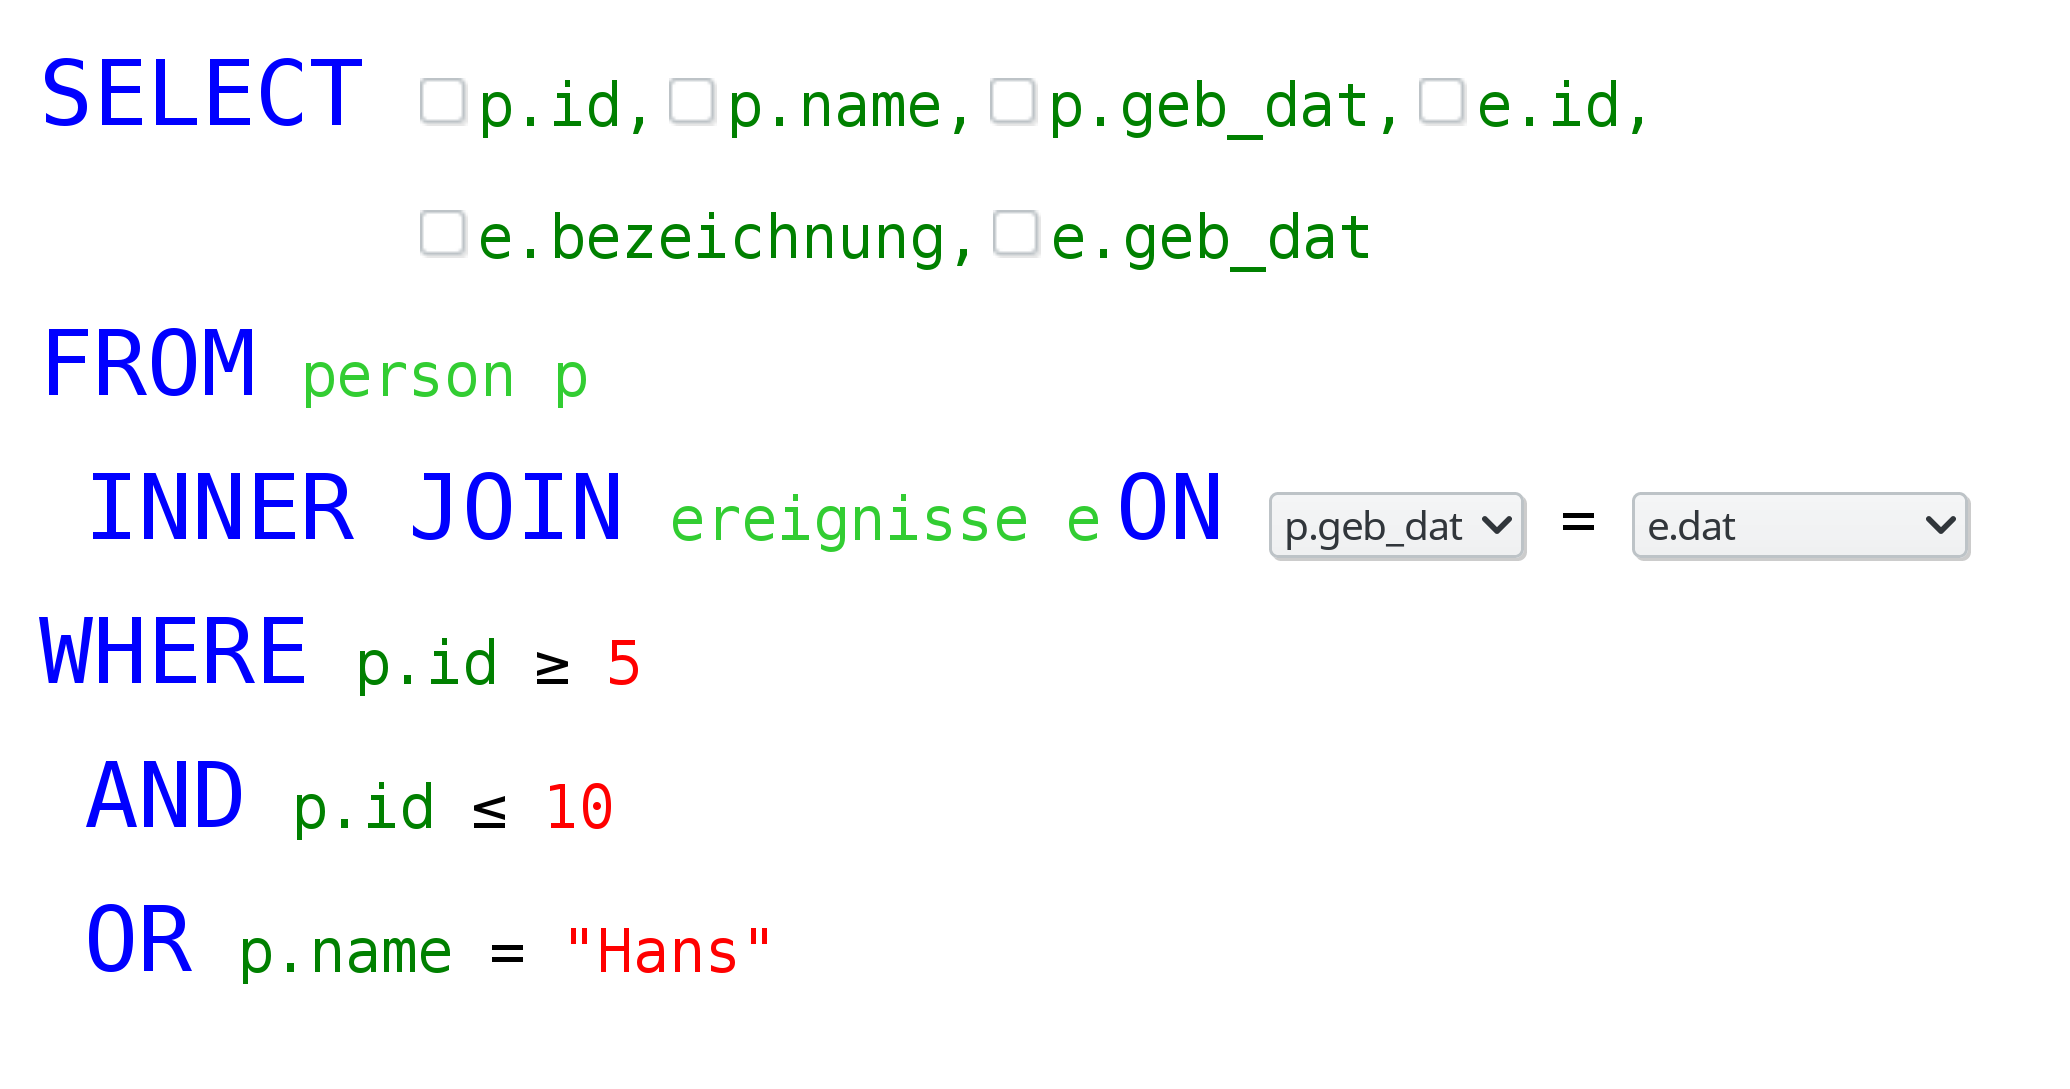
\includegraphics[width=\textwidth]{images/sql-sketch-early-syntax-highlight}
    \caption{Syntax-Highlighting, ähnlich einer IDE}
    \label{fig:screen-sql-editor-early-syntax-highlighting}
  \end{subfigure}
  \caption{Vergleich unterschiedlicher Gestaltungsansätze}
  \label{fig:compare-colourful}
\end{figure}

\subsubsection{Grundsätzlicher Aufbau des Editors}

Es stellt sich also die Frage, ob der Editor, wie Scratch, mit einer Drag \& Drop Seitenleiste ausgestattet werden sollte, oder ob auch ein anderes Bedienkonzept denkbar wäre. Ein grundsätzlicher Nachteil Drag \& Drop Bedienkonzeptes ist der nötige Platz für die Unterbringung aller verwendbaren Komponenten. Spätestens wenn für die Anzeige aller verfügbaren Optionen nicht ausreichend Platz auf dem Bildschirm vorhanden ist, muss sorgfältig geplant werden, wie die Bedienelemente anzuordnen sind.

Da der Benutzer immer nur eine Abfrage zur Zeit bearbeiten können soll, ergibt sich der einzig mögliche Platz für viele Blöcke automatisch. Darüber hinaus ist die Reihenfolge eines Großteils der Komponenten einer Abfrage sehr strikt festgelegt, so kann eine \texttt{GROUP BY} Komponente nicht an beliebigen Stellen verwendet werden, sondern nur nach der \texttt{FROM} oder der \texttt{WHERE} Anweisung. Andere Komponenten wie z.B. \texttt{HAVING} oder logische Verknüpfungen mit \texttt{AND} oder \texttt{OR} sind nicht nur von der Reihenfolge, sondern auch von der Existenz anderer Bestandteile abhängig. Ein möglicher Ansatz wäre also, die möglichen Optionen visuell abgegrenzt Platzhalter innerhalb des Abfrageeditors anzubieten. Ein Klick auf den Platzhalter wandelt diesen dann in einen konkreten Block um und fordert ggfs. zur Angabe der benötigten Parameter auf.

\begin{wrapfigure}{r}{0.46\textwidth}
  \includegraphics[width=0.45\textwidth]{images/sql-sketch-all-editing}
  \caption{So nicht! Simultane Anzeige (fast) aller Möglichkeiten}
  \label{fig:screen-sql-editor-all-editing}
\end{wrapfigure}

Im Rahmen der entwickelten Prototypen hat sich herausgestellt, dass eine permanente Anzeige aller Editierungsmöglichkeiten mit einem sehr überladen wirkenden Benutzerinterface einher geht, insbesondere was die Einblendung von Platzhaltern angeht. Abbildung \ref{fig:screen-sql-editor-all-editing} zeigt einen Screenshot des Prototypen, bei dem nahezu alle denkbaren Editierungsoptionen gleichzeitig für den Lernenden verfügbar sind und daher angezeigt werden müssen. Trotz der klaren visuellen Unterscheidung fällt es schwer mit nur einem Blick zu erkennen, was die Abfrage jetzt tatsächlich beinhaltet. Statt jederzeit alle Optionen anzuzeigen wurde dann noch die Position des Mauszeigers herangezogen um zu entscheiden, welche Platzhalter angezeigt werden sollen. Das Ergebnis war allerdings eine Benutzerschnittstelle, deren Bedienelemente häufig und für einen ungeübten Benutzer auch unerwartet ihre Position verändert haben. Dementsprechend wurde dieser Ansatz noch in der Konzeptionsphase verworfen.

Das endgültig implementierte Design (Abbildung \ref{fig:screen-sql-editor-drag-drop}) lehnt sich nun doch an Scratch an, versucht allerdings mit Platzhaltern den Benutzer kontextsensitiv zu unterstützen. Wenn dieser zum Beispiel einen Vergleichsoperator für Ausdrücke in der Seitenleiste anwählt, werden im Hauptfenster die validen Drop-Ziele hervorgehoben. Unter dem eigentlichen Editor befinden sich dann zwei weitere Bereiche (Abbildung \ref{fig:screen-sql-editor-parameters-preview}): Zum einen die Ergebnisanzeige, welche die zur aktuellen Gestalt der Abfrage passenden Zeilen zeigt. Und zum anderen eine Möglichkeit, bei Abfragen mit Parametern die nötigen Werte zu definieren. Und an dieser Abbildung wird ein weiteres Detail deutlich: Abfragen lassen sich nur als "`einzeilig"' deklarieren, wenn eine \texttt{WHERE}-Komponente vorhanden ist.

\begin{figure}[h]
  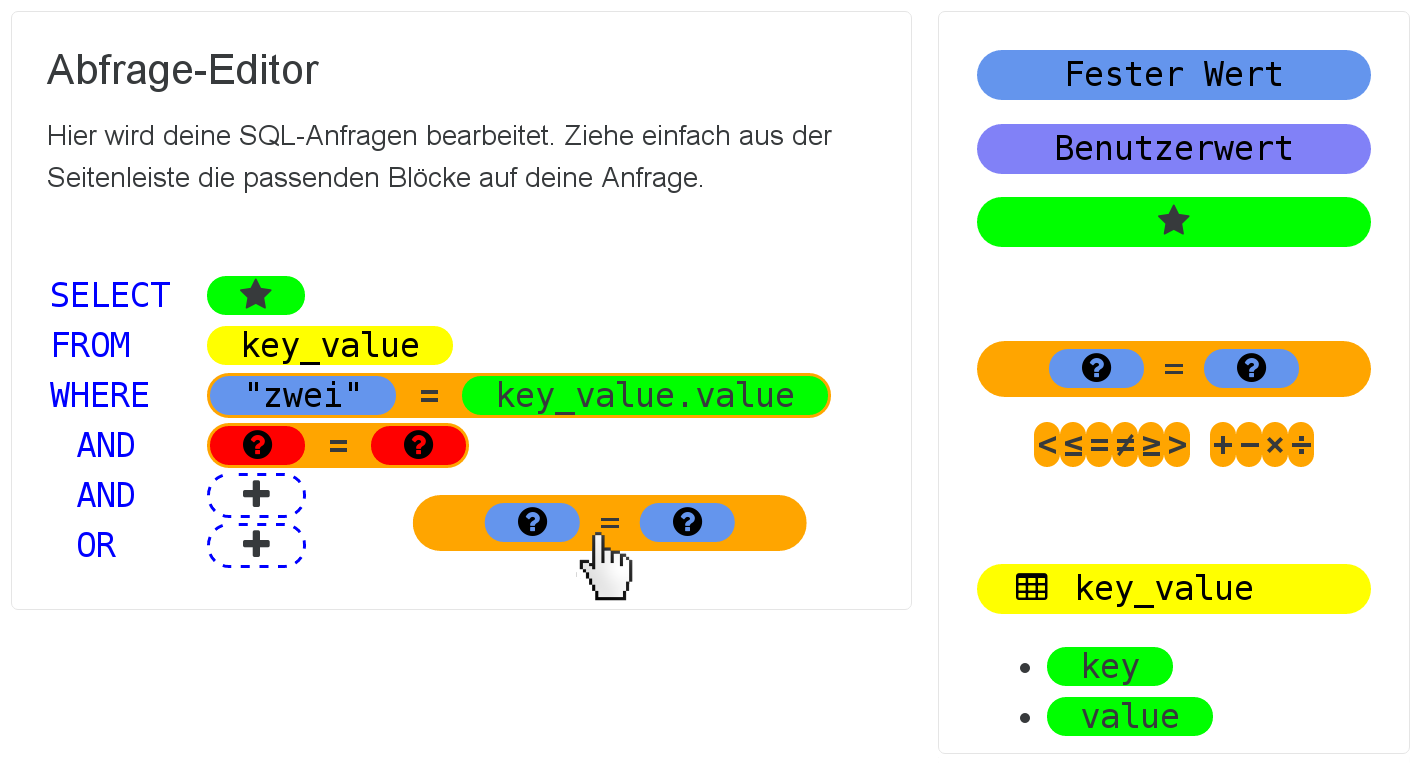
\includegraphics[width=\textwidth]{images/sql-drag-drop}
  \caption{Abfrageeditor: Drag \& Drop Interface mit Hervorhebung von möglichen Zielen beim Ziehen aus der Seitenleiste}
  \label{fig:screen-sql-editor-drag-drop}
\end{figure}
  
\begin{figure}[p]
  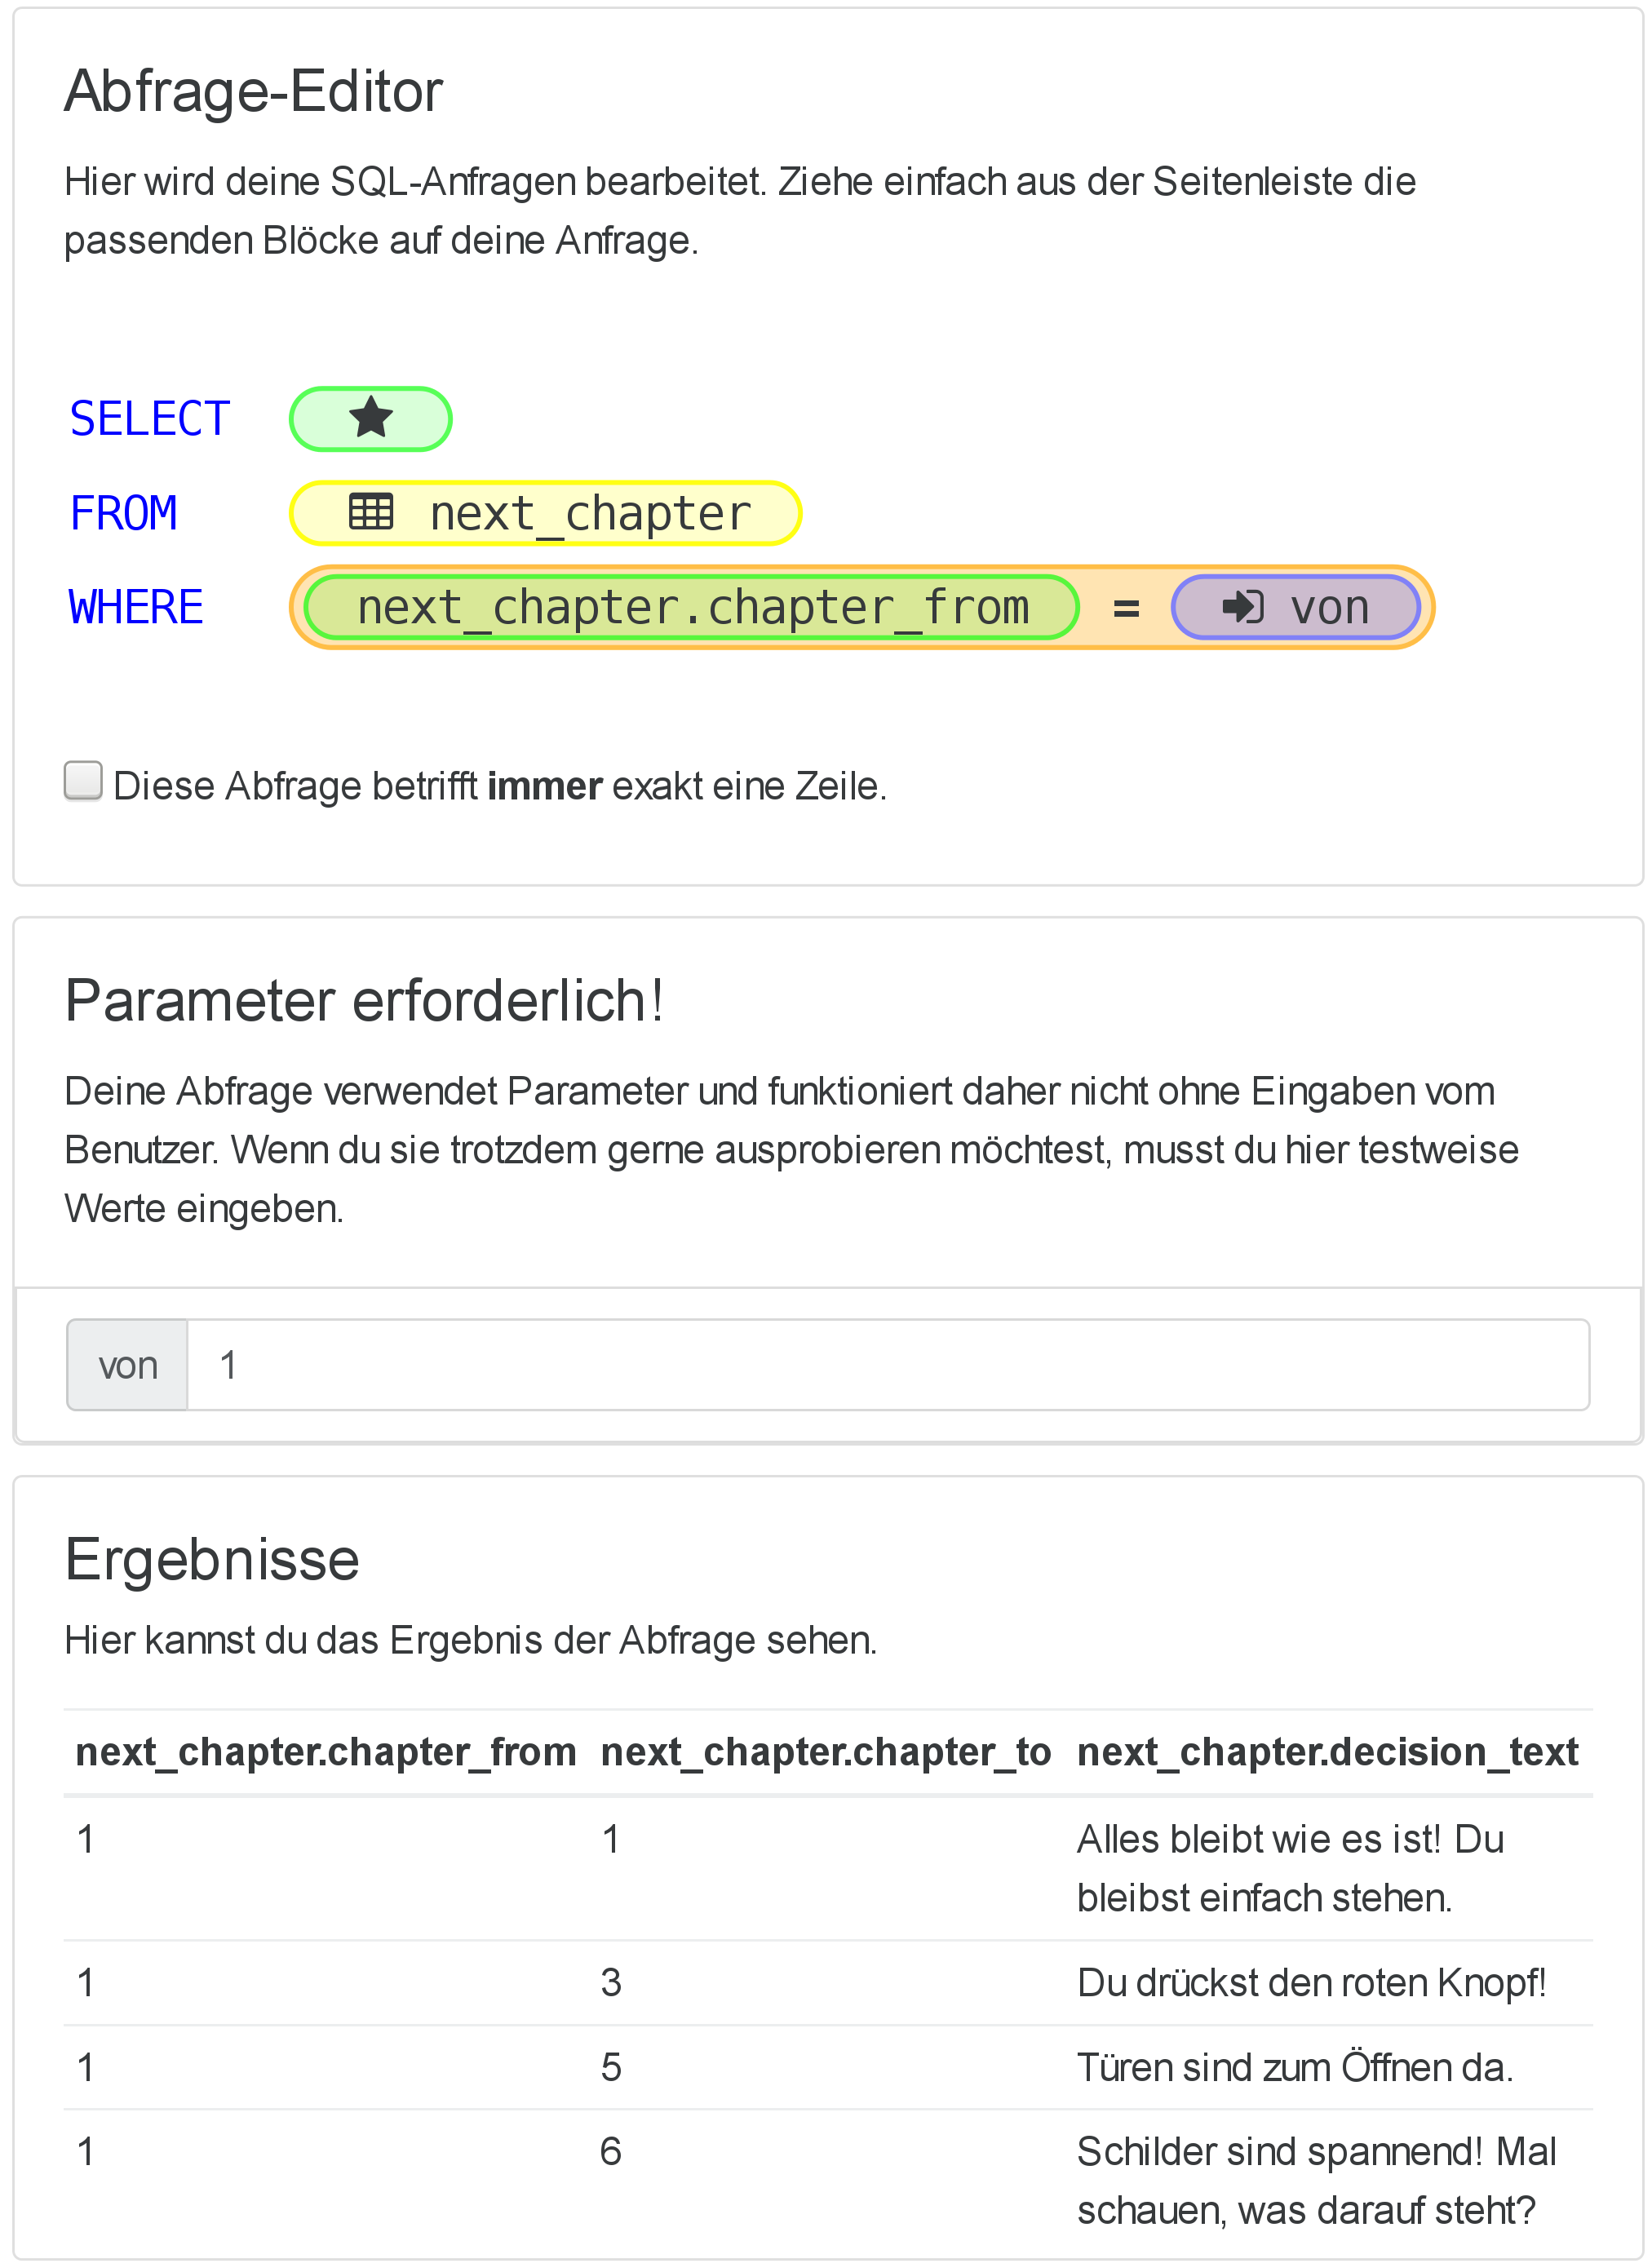
\includegraphics[width=\textwidth]{images/sql-parameters-preview}
  \caption{Abfrageeditor: Parameter für eine parametriesierte Abfrage und Ergebnisvorschau}
  \label{fig:screen-sql-editor-parameters-preview}
\end{figure}


\todo[inline]{Perspektivisch interessant wäre an dieser Stelle noch die Hervorhebung in die andere Richtung: Wenn man mit der Maus über eine SQL-Komponente im Editorfenster verweilt, werden die möglichen Optionen in der Seitenleiste hervorgehoben.}

\subsubsection{\texttt{SELECT}}

\subsubsection{\texttt{JOIN}}

Wenn der Benutzer eine Drag-Operation mit einer Tabelle beginnt, kann er die Tabelle wahlweise auf einer bestehenden Tabelle "`fallen lassen"', einen $\bigoplus$-Indikator nach der letzten Tabelle oder den \texttt{FROM}-Text selbst fallen lassen. Eingefügt wird dabei im Falle von schon existierenden Elementen immer nach dem Ziel, Indikatoren werden einfach durch das neue Element ersetzt.

\subsubsection{\texttt{WHERE}}

\subsubsection{\texttt{GROUP BY}}

Sobald in einer Abfrage eine \texttt{GROUP BY} Komponente auftaucht, hat dies Auswirkungen auf die Möglichkeiten innerhalb der \texttt{SELECT} Anweisung. Da keine Auswahl von ungruppierten und nicht-aggregierten Spalten möglich sein darf, müssen diese entfernt werden. Insbesondere wenn der Benutzer vorher schon mit komplizierten Ausdrücken im \texttt{SELECT} gearbeitet haben sollte, ist also zumindest eine Warnung nötig.

\subsubsection{Abfragen mit Parametern}
\label{sec:design-query-params}

Um eine Interaktion mit Endbenutzern zu ermöglichen können in Abfragen auch benannte Parameter anstelle von konstanten Werten verwendet werden. Diese müssen dann zur Laufzeit vom Benutzer angegeben werden. Aus Sicht der SQL-Abfrage ist diese Ergänzung relativ trivial, schließlich sind benannte Parameter Teil faktisch jeder SQL-Implementierung. Die eigentliche Problematik liegt im Binden dieser Parameter zur Laufzeit. Das Kapitel \ref{sec:design-ui-editor} beschreibt den Editor für Benutzeroberflächen, durch welchen die Verknüpfung mit den Bedienelementen der Oberfläche vorgenommen wird.

\subsubsection{Manipulation von Daten}

Neben den bisher ausführlich besprochenen \texttt{SELECT}-Anweisungen müssen sich natürlich \texttt{INSERT}-, \texttt{UPDATE}- und \texttt{DELETE}-Anweisungen umsetzen lassen. Da diese ihrer Natur nach nicht idempotent sind verbietet sich natürlich eine wiederholte, automatische Ausführung während der Entwicklungszeit.

\todo[inline]{Vorschau für Manipulationen}

Für die Name-Wert-Paare in \texttt{INSERT} oder \texttt{UDPATE} Operationen löst sich das Erscheinungsbild des Editors von dem Vorbild der SQL-Sprache (Abbildung  \ref{fig:screen-sql-editor-insert-key-value-pairs}).

\begin{figure}[h]
  \includegraphics[width=\textwidth]{images/sql-insert-key-value-pairs}
  \caption{Abfrageeditor: Anderes Erscheinungsbild für Spalte-Wert-Paare, wie sie bei \texttt{INSRT} oder \texttt{UPDATE} Operationen nötig sind}
  \label{fig:screen-sql-editor-insert-key-value-pairs}
\end{figure}

Es ist zu erwarten, dass die meisten von den Schülern verfassten Abfragen dieser Art ausführlichen Gebrauch von den in Kapitel \ref{sec:design-query-params} beschriebenen Parametern machen.

\subsection{Konzept für Oberflächen}
\label{sec:design-ui-concept}

\warning{Diese Oberflächen werden nicht ausschließlich in normalem HTML verfasst, es kommen noch einige Erweiterungen in Form einer Templatingengine zum Einsatz. Ähnlich wie für die SQL-Abfragen wird also auch für die Oberflächen ein dezidierter Editor (Kapitel \ref{sec:design-ui-editor}) implementiert. Die Schüler sollten zu keinem Zeitpunkt selber Quelltexte tippen müssen, optional aber durchaus die Möglichkeit dazu haben.}

Damit sich mit der Schülerentwicklungsumgebung erstellte Projekte auch von normalen Endanwendern bedienen lassen können Bedarf es natürlich einer entsprechenden Benutzeroberfläche. Hier bietet sich aus Gründen der einfachen Weitergabe eine webbasierte Oberfläche an: So entfällt bei den Endanwendern jegliche Installation und gerade für datenzentrierte, verteilte Anwendungen ist eine einheitliche Sicht auf den Datenbestand von großer Bedeutung.

\subsubsection{Die Templatingsprache Liquid}

Auch wenn die Schüler mit der Syntax der verwendeten Templatingsprache nur so wenig möglich in Berührung kommen sollten lohnt sich eine kurze Betrachtung der Syntax dieser Sprache. Grundsätzlich unterschieden wird in Liquid zwischen drei verschiedenen Anweisungen \cite{liquid-introduction}:

\begin{description}
\item[Objekte] \hfill \\
  Objekte werden in doppelt geschweiften Klammern notiert (also \texttt{\{\{Objekt\}\}}) und erlauben Zugriff auf einen hinterlegten Datenbestand. 
\item[Tags] \hfill \\
  Tags steuern den Programmfluss.
\item[Filter] \hfill \\
  Anwendung von Funktionen auf bestehende Daten.
\end{description}

\subsubsection{Layout}

Eine immer wiederkehrende Frage bei der Entwicklung von Webseiten ist die nach dem Layout der gesamten Seite. Technisch gesehen erfolgt die Umsetzung des Layouts heutzutage über eine Vielzahl unterschiedlicher CSS-Direktiven, deren Erstellung keinesfalls ein Kernbereich der Entwicklungsumgebung ist. Allerdings lassen sich auf den meisten Seiten immer wiederkehrende Strukturen feststellen: Die Unterteilung der Seite in ein Raster aus Zeilen und Spalten, Abbildung \ref{fig:grid-example} zeigt ein solches Layout. Dort werden die beiden obersten Zeilen für den Header und die Pfadangabe nicht weiter in Spalten unterteilt, bestehen technisch gesehen also aus einer einzigen, sehr breiten Spalte. Die dritte Zeile enthält drei Spalten (Navigation, Inhalt und eine Leiste für Module), wobei diese letzte Modulspalte wiederum mehrere Zeilen enthält.

\begin{figure}[p]
  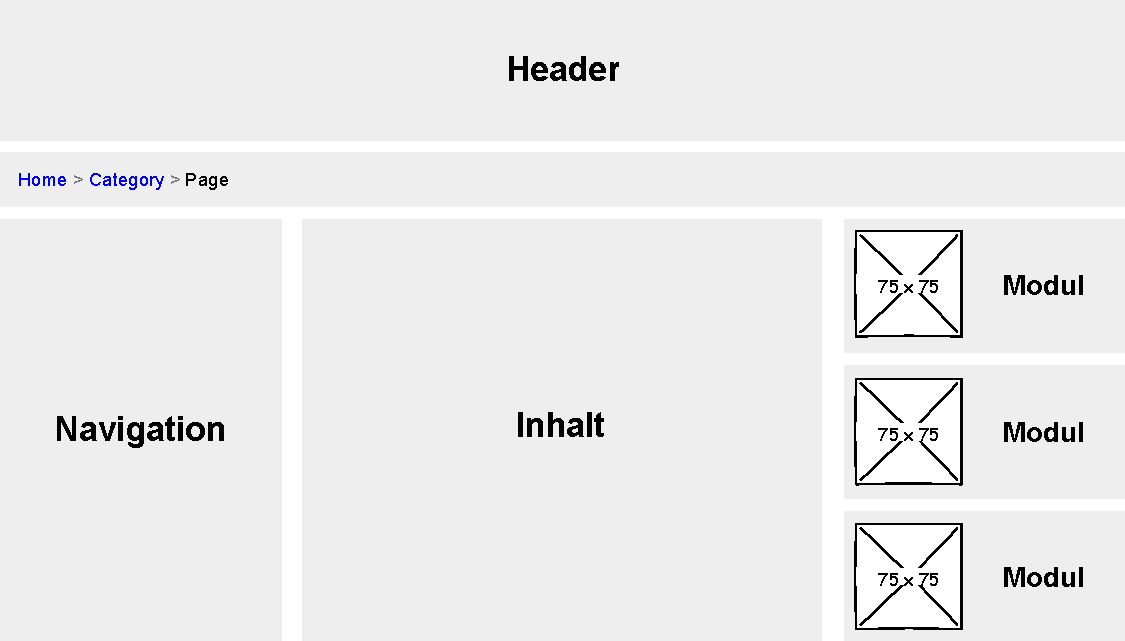
\includegraphics[width=\textwidth]{sketches/grid-example}
  \caption{Seite mit einem Raster aus Zeilen und Spalten}
  \label{fig:grid-example}
\end{figure}

Diese Layoutstruktur wird mittlerweile von einer Vielzahl von vorhandenen CSS-Bibliotheken unterstützt und soll auch das grundsätzliche Gedankenmodell für die hier beschriebenen Oberflächen sein. Es ergeben sich daraus die folgenden Layoutelemente:

\begin{description}
\item[Zeilen] \hfill \\
  Zeilen enthalten eine oder mehrere Spalten, wobei jeder Inhalt zwingend in einer Spalte platziert werden muss. Die Höhe einer Zeile entspricht der Höhe der höchsten Spalte.
\item[Spalten] \hfill \\
  Die Breite einer Spalte wird in einem relativen Maß mit Bezug zu einer bestimmten Bildschirmgröße angegeben. So können für breite Bildschirme z.B. drei Spalten vorgesehen werden, für sehr schmale Geräte wie Smartphones hingegen nur eine Spalte. Sollte die Summe dieser Breitenangaben der Spalten die maximale Breite einer Zeile überschreiten, werden diese auf mehrere Zeilen umgebrochen.
\end{description}

\missing[inline]{Visuelles Beispiel für den Umbruch}

\subsubsection{Bedienelemente}

Grundsätzlich lassen sich alle Bedienelemente anhand der Struktur von Ein- und Ausgaben unterscheiden (Abbildung \ref{fig:ui-element-concept}). Die Unterscheidung, ob eine Ein- bzw. Ausgabe exakt einen Wert oder alternativ mehrere (oder keinen) Wert erwartet bzw. liefert ist für die Oberfläche von zentraler Bedeutung. Die Kapitel \ref{sec:design-ui-bind-output} \nameref{sec:design-ui-bind-output} und \ref{sec:design-ui-bind-input} \nameref{sec:design-ui-bind-input} erläutern diese Unterscheidung noch einmal ausführlich.

\begin{figure}[p]
  \centering \begin{tikzpicture}
  \tikzset{square matrix/.style={
      column sep=-\pgflinewidth, row sep=-\pgflinewidth,
      nodes={
        minimum height=#1,
        anchor=center,
        text width=#1,
        align=center,
        inner sep=6pt
      },
    },
    square matrix/.default=3.50cm
  }


  \matrix[square matrix] (my matrix) at (0,0)
  {
    \node (single)   {Unmittelbare Ausgabe, z.B. in einem Text}; &
    \node (passive)  {Einfaches Eingabelement, z.B. eine Textbox}; \\
    \node (multiple) {Wiederholte Ausgabe, z.B. eine Tabelle}; &
    \node (input)    {Eingabelement mit Mehrfachauswahl}; \\
  };
  \draw [thick,-] (my matrix.east)  |- (my matrix.west);
  \draw [thick,-] (my matrix.south) |- (my matrix.north);

  \node [left=of single, anchor=north, rotate=90] {\textsc{Eine Zeile}};
  \node [left=of multiple, anchor=north, rotate=90] {\textsc{Beliebig}};
  \node [above=of single, anchor=north] {\textsc{Keine Eingabe}};
  \node [above=of passive, anchor=north] {\textsc{Eingabe}};
\end{tikzpicture}



%%% Local Variables:
%%% mode: latex
%%% TeX-master: "../thesis"
%%% End:

  \caption{Einordnung von Bedienelementen}
  \label{fig:ui-element-concept}
\end{figure}

Zwar sollen im Regelfall keine komplett statischen Seiten angezeigt werden, trotzdem muss es natürlich eine Möglichkeit geben statische Texte ohne Bindung an irgendwelche Abfragen zur Anzeige zu bringen. Die hier vorgestellten Bedienelemente funktionieren auch ohne jede Datenquelle, die folgenden Kapitel stellen aber noch Erweiterungen zur Datenanbindung vor.

\begin{description}
\item[Überschriften] \hfill \\
  HTML sieht die Verwendung von Überschriften in sechs Hierarchiebenen vor und stellt dafür distinkte Elemente zur Verfügung (\texttt{<h1>} bis \texttt{<h6>}). Dieser Umstand soll nicht unmittelbar abgebildet werden. Stattdessen gibt es ein allgemeines Bedienelement ``Überschrift'', zu dem sich dann eine Ebene auswählen lässt.
\item[Absätze] \hfill \\
  Blöcke von zusammenhängendem Text werden als Absatz ausgezeichnet, das entsprechende HTML-Äquivalent ist das \texttt{<p>}-Element.
\item[Listen] \hfill \\
  Strukturiert zusammenhängende Daten werden als sortierte oder unsortierte Liste (\texttt{<ol>} bzw. \texttt{<ul>} in HTML) gruppiert. Wie schon bei den Überschriften soll an dieser Stelle nur ein logisches Listenelement zum Einsatz kommen, dass dafür über eine Eigenschaft ``Nummerierung'' verfügt.      
\item[Bilder] \hfill \\
  Zwar technisch betrachtet ein eher simples Unterfangen, für Schüler erfahrungsgemäß aber motivierend, ist die Einbindung von Bildern. Diese entsprechen einem HTML \texttt{<img>}-Element, für welches das \texttt{src}-Attribut gesetzt werden muss.
\end{description}

Spätestens durch die Aufnahme von Bildern ist auch für statische Webseiten eindeutig, dass es möglich sein muss diese Bedienelemente über die Angabe von Parametern zu beinflussen. In den meisten Fällen werden diese Parameter zur Laufzeit durch die Ausführung einer Abfrage mit konkreten Werten bestückt, die Angabe von konstanten Werten ist aber ebenfalls möglich.

\subsubsection{Bindung von Daten an die Oberfläche}
\label{sec:design-ui-bind-output}

Ein Großteil der Oberflächenelemente wird also einige Eigenschaften aufweisen, deren Inhalte erst zur Laufzeit dynamisch gebunden werden. Dabei stellt sich die Frage, wie die Struktur der zur Verfügung stehenden Daten eigentlich definiert wird bzw. aussehen soll?

Auf abstrakter Ebene ist die Beantwortung dieser Frage eindeutig: Da das Ergebnis einer SQL-Abfrage grundsätzlich eine Tabellenstruktur mit Zeilen, Spalten und Zellen ist, wird dieses Datenmodell auch für die Oberfläche zugrunde gelegt. Die an die Bedienelemente zu bindenden Daten sind also grundsätzlich tabellarischer Natur.

Um im Falle von mehreren in Frage kommenden Abfragen eine eindeutige Zuordnung vornehmen zu können, müssen Abfragen, deren Ergebnis an die Oberfläche gebunden werden soll, mit einem eindeutigen Namen bezeichnet werden. Dieser Name kann von den Entwicklern frei gewählt werden, sollte aber, analog zu einem Funktionsbezeichner, sinnvoll darüber Auskunft geben was eine Abfrage bewirkt. Der Umgang mit den Zeilen erfordert keine Sonderbehandlung, hier genügt die Angabe eines Zeilenindex. Für die Spalten entfällt glücklicherweise eine ``künstliche'' Benennung, diese werden trivialerweise über ihren Namen entsprechend der \texttt{SELECT}-Komponente angesprochen. Mit diesen drei Werten (Name der Abfrage, Zeilenindex, Spaltenname) lässt sich jede Zelle einer Menge von Abfragen eindeutig identifizieren.

Aus praktischen Gründen sollten Abfragen allerdings bezüglich der Anzahl der erwarteten Zeilen annotiert werden können, konkret unterschieden werden muss dabei zwischen ``exakt eine Zeile'' und ``beliebig viele (auch keine) Zeilen''. Im Falle einer Abfrage mit nur einer Zeile entfällt dann Notwendigkeit einen Zeilenindex anzugeben, dieser bezieht sich trivalerweise immer auf die einzige, zur Verfügung stehende Zeile. Wenn Daten an die Oberflächen gebunden werden entfällt durch diese Abkürzung die permanente Angabe einer redundanten Information.

Listing \ref{lst:sql:person-days} zeigt eine Abfrage die in Listing \ref{lst:html:person-days-index} und \ref{lst:html:person-days} einmal mit und einmal ohne Index gebunden wird. Das ist zwar ein kleiner Vorgriff, demonstriert aber wie diese Annotation der Lesbarkeit zu gute kommt.

\begin{lstlisting}[language=SQL, caption=Abfrage mit garantiert einer Ergebniszeile,label=lst:sql:person-days]
SELECT name, geburtstag
FROM   person
LIMIT  1;
\end{lstlisting}

\begin{lstlisting}[language=HTML, caption=String-Interpolation mit Indexzugriff, label=lst:html:person-days-index]
<!-- benutzer = Listing (*@\ref{lst:sql:person-days}: \nameref{lst:sql:person-days}@*) -->
<p>Hallo {{ benutzer[0].name }}, du bist am {{ benutzer[0].geburtstag }} geboren.</p>
\end{lstlisting}

\begin{lstlisting}[language=HTML, caption=String-Interpolation mit implizitem Index, label=lst:html:person-days]
<!-- benutzer = Listing (*@\ref{lst:sql:person-days}: \nameref{lst:sql:person-days}@*) -->
<p>Hallo {{ benutzer.name }}, du bist am {{ benutzer.geburtstag }} geboren.</p>
\end{lstlisting}

Diese Annotation muss jedoch vom Entwickler manuell gesetzt werden, eine automatische Berechnung wäre für beliebige Abfragen unmöglich\footnote{Viele SQL-Dialekte sind Turing-Vollständig und schon das Halteproblem ist nicht entscheidbar.} und auch für speziell strukturierte Abfragen ist diese Unterscheidung zumindest nicht trivial. Oder um es anders auszudrücken: Die Erweiterung der Entwicklungsumgebung um diese automatische Vorhersage wäre Stoff für eine weitere wissenschaftliche Arbeit, keinesfalls aber Gegenstand dieser Arbeit. Praktischerweise lässt sich eine auftretende Verletzung dieser Annotation aber sehr gut erkennen und daher auch sinnvoll an den Entwickler kommunizieren. Und letzten Endes könnte ein Entwickler die Garantie durch die Einführung einer \texttt{LIMIT 1}-Komponente selber geben, was möglicherweise aber zu überraschendem Verhalten zur Laufzeit führt.

Diese gesonderte Behandlung von bestimmten Tabellendimensionen ist übrigens keine Erfindung dieser Thesis: Auch SQL selbst hebt einige Abfragen mit speziellen Strukturen hervor. Tabellen mit nur einer Zelle können als skalarer Wert eingesetzt werden, bei nur einer Spalte können Abfragen z.B. für \texttt{IN}-Ausdrücke verwendet werden.

Der Umgang mit den Zeilen einer Abfrage ist im Rahmen der Oberfläche ein bisschen komplizierter, da hier technisch gesehen häufig zwei verschiedene Elemente zum Einsatz kommen müssen: Ein Containerelement und ein sich wiederholendes Element. Auch an dieser Stelle tätigen wir daher mit Listing \ref{lst:sql:people-days} und \ref{lst:html:people-days} einen kurzen Vorgriff, um den grundsätzlichen Unterbau zu demonstrieren.

\begin{lstlisting}[language=SQL, caption=Abfrage mit beliebig vielen Ergebniszeilen,label=lst:sql:people-days]
SELECT name, geburtstag
FROM   person;
\end{lstlisting}

\begin{lstlisting}[language=HTML, caption=Containerelemente mit Kindern, label=lst:html:people-days]
<!-- alleBenutzer = Listing (*@\ref{lst:sql:people-days}: \nameref{lst:sql:people-days}@*) -->
<ul>
  
    <li>
      {{ benutzer.name }} wurde am {{ benutzer.geburtstag }} geboren.
    </li>
  
</ul>
\end{lstlisting}

\subsubsection{Eingabe von Daten über die Oberfläche}
\label{sec:design-ui-bind-input}

Immer wenn eine Abfrage mit Platzhaltern an eine Seite gebunden wird, ist es notwendig dem Benutzer eine Möglichkeit zu geben diese Platzhalter zu füllen. Im einfachsten Fall kann diese Bindung über einfache \texttt{<input type=text>}-Elemente hergestellt werden. Das ist für viele Arten von Such- und Eingabemasken auch sicherlich ausreichend, führt jedoch zu Problemen bei Beziehungen zwischen Entitäten. In diesem Fall müsste in das Textfeld vom Benutzer ein Primärschlüssel angegeben werden, was ganz sicher kein besonders Benutzerfreundliches Konzept darstellt.

In einem solchen Fall soll es also möglich sein auch Bedienelememente wie Comboboxen zu verwenden, die ihrerseits wieder eine Abfrage zur Anzeige der zur Verfügung stehenden Daten benötigen. Dabei muss klar zwischen zwei benötigten Informationen unterschieden werden. Auf der einen Seite muss das Resultat eines solchen Bedienelements vermutlich einen Primärschlüssel zurückliefern. Auf der anderen Seite erwarten die Benutzer aber die Anzeige von ``intuitiven'' Informationen, anhand derer Sie ihre Auswahl treffen können. Der Primärschlüssel ist typischerweise eine künstliche Spalte, die für den Endanwender keinerlei Informationsgehalt hat. Praktischerweise ist auch diese Unterscheidung in HTML vorgesehen

\begin{lstlisting}[language=HTML, caption=Containerelemente mit Kindern, label=lst:html:select-example]
<!-- alleBenutzer = Listing (*@\ref{lst:sql:people-days}: \nameref{lst:sql:people-days}@*) -->
<select>
  
    <option value="{{ benutzer.id }}">
      {{ benutzer.name }}
    </option>
  
</select>
\end{lstlisting}

\subsubsection{Seitenstruktur und Navigation}

Zunächst ist festzuhalten, dass die serverseitige Erzeugung von Seiten zur Laufzeit nicht vorgesehen ist. Stattdessen definiert der Entwickler eine Reihe von serverseitig statischen HTML-Seiten samt einiger Datenquellen, die dann vom Client des Anwenders ausgeführt werden. Der Client analysiert dann zunächst die in der Seite hinterlegten Datenquellen und führt ggfs. weitere HTTP-Anfragen aus, um alle Daten einzusammenln.

Die Seiten können beliebig in einer Ordnerstruktur organisiert werden, die Dateipfade bilden nicht die Grundlage für das Routing. Diese Entkoppelung der Pfade im Dateisystem von den URLs erlaubt es den Schülern die Übergabe von Parametern und auch die sonstige Navigationsstruktur frei zu gestalten.

Zu jeder dieser Seiten können eigene Datenquellen hinterlegt werden. Dabei sind bisher die folgenden Möglichkeiten vorgesehen:

\begin{description}
  \item[Parameter aus URLs] \hfill \\
    Zur Übergabe von Informationen zwischen Seiten können Teile der URL als Parameter für die Seite markiert werden.
  \item[Abfragen] \hfill \\
    Die ``typische'' Datenquelle für Seiten.
  \item[Variablen \& Konstanten] \hfill \\
    Manchmal kann es nötig sein, verschiedene Konstrukte ohne eine Datenbank im Hintergrund zu erproben. In diesem Fall bietet sich die Verwendung von vordefinierten Werten an.
\end{description}

Damit für jede Seite eindeutig ist, über welche kanonischen URLs sie angesprochen werden kann muss der Entwickler eine Routing-Konfiguration hinterlegen. In dieser wird einem einfachen Pfad, ggfs. auch mit Platzhaltern für Parameter, ein eindeutiger Name sowie eine anzuzeigende HTML-Seite zugewiesen. Der Name ist nötig um, unabhängig von einer sich möglicherweise ändernden Pfadangabe, ein eindeutiges Ziel für Links angeben zu können. Nur wenn diese Eindeutigkeit hergestellt ist, kann der Entwickler auf z.B. nicht existierende Linkziele oder fehlende Parameter hingewiesen werden.

Für einen einfachen Blog wäre z.B. die folgende interne Repräsentation der Konfiguration denkbar:

\begin{lstlisting}[language=JavaScript, caption=Einfache Routen für einen Blog, label=lst:json:simple-routing-blog]
{ path : "/",            name : "Hauptseite", page : "index.html",
  path : "/beitrag/:id", name : "Beitrag",    page : "beitrag.html" }
\end{lstlisting}

\subsection{Editor für Oberflächen}
\label{sec:design-ui-editor}

Der Editor für Oberflächen nimmt die Konzepte aus dem vorigen Kapitel und macht sie den Entwicklern auf eine intuitive Art zugänglich. Abbildung \ref{fig:ui-editor-sketch-first} zeigt den grundsätzlichen Aufbau der Oberfläche aus einem zentralen Designbereich und einer Seitenleiste. Die Verbindungen zwischen den Bedienelementen und den Daten aus der Seitenleiste verdeutlichen zu Illustrationszwecken deren Zusammenhang. In der endgültigen Fassung des Editors soll der Zusammenhang nicht durch Linien dargestellt werden, sondern durch einen Hervorhebungseffekt wenn einer der beiden Seiten aktuell ausgewählt ist.

\unsure[inline]{Eigentlich würde ich gerne auf Tabs in der Seitenleiste verzichten, die Daten könnte man ja auch innerhalb des Designbereiches darstellen. Diesen Weg der Platzierung von nicht sichtbaren Elementen hat auch schon die Delphi IDE betreten und so dramatisch schlimm fand ich das nicht.}

\begin{figure}[h]
  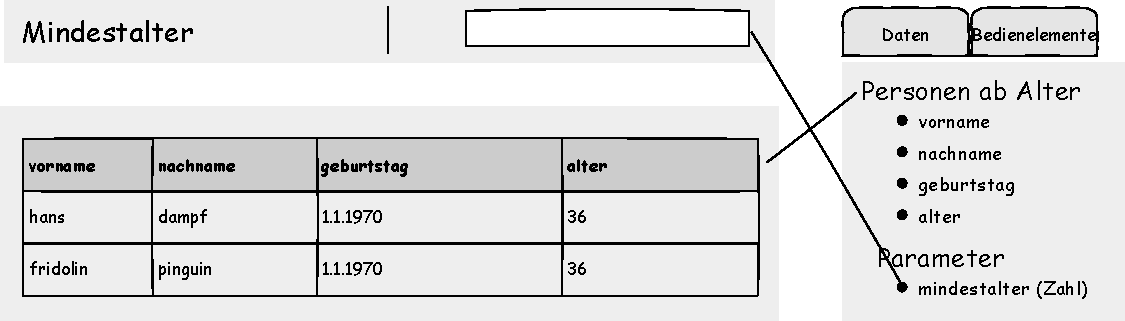
\includegraphics[width=\textwidth]{sketches/ui-sketch-first}
  \caption{Skizze des Oberflächeneditors mit Tabs}
  \label{fig:ui-editor-sketch-first}
\end{figure}

Wenn der Benutzer auf den Tab für die Bedienelemente wechselt, bekommt er eine Übersicht aller verfügbaren Bedienelemente. Diese können dann per Drag \& Drop auf dem Designbereich platziert werden. Einige Bedienelemente verfügen über komplexere Eigenschaften, diese werden dann separat dargestellt.

\unsure[inline]{Ich bin noch absolut unentschlossen, wie bzw. wo ich die weiteren Eigenschaften von komplexen Eigenschaften unterbringen soll. Die ``klassische'' Variante aller aktuellen Entwicklungsumgebungen ist eine weitere Seitenleiste, die hätte dann in diesem Fall dann allerdings drei Tabs. Daher überlege ich alternativ möglichst viele Informationen unmittelbar im Designbereich unterzubringen. Wenn man dann ein Bedienelement anklickt klappt sich darunter (oder sonstwo) ein Bereich auf, in dem die weiteren Einstellungen vorgenommen werden können.}

\subsection{Beispielhafte Datenbasen}
\label{sec:example-queries}

%%% Local Variables:
%%% mode: latex
%%% TeX-master: "thesis"
%%% End:
